%=============================================================================
\documentclass[10pt,a4paper]{article}
%
%
%
\usepackage{graphicx}
\usepackage{hyperref}
\usepackage{verbatim}
\usepackage{fix-cm}
\usepackage{lineno}
\usepackage{fancyhdr}
%
\usepackage{amsmath}
%
\oddsidemargin  0.1 in
\evensidemargin 0.1 in
%
%
\newlength{\backindent}\setlength{\backindent}{2cm}
\textwidth 5.375 in % Width of text line.
\advance\textheight by1.4cm
\advance\voffset by-1.4cm
\advance\textwidth by\backindent
%
%
% === Fancy headers setup  ===============================
%
\setlength{\headheight}{15.2pt}
\pagestyle{fancyplain} {
\fancyhead[L]{
\includegraphics[height=10mm]{DD4hep-AIDA-logo.png}\vspace{-0.3cm}}
\fancyhead[C]{}
\fancyhead[R]{\sffamily{\underline{\hspace{6cm}Advanced European Infrastructures for Detectors at Accelerators}}}
\fancyfoot[L]{}
\fancyfoot[C]{\sffamily{User Manual}}
\fancyfoot[R]{\sffamily{\thepage}}
}
%
%
\newcommand{\tw}[1]{${\tt{#1}}$}
\newcommand{\tts}[1]{{\tt\small{#1}}}
\newcommand{\bold}[1]{{\bf{#1}}}
%
%
\newcommand{\DDE}{{$\tt{DDEve}$\space}}
\newcommand{\DDhep}{{$\tt{DD4hep}$\space}}
\newcommand{\DDH}{{$\tt{DD4hep}$\space}}
\newcommand{\DDG}{{\tt{DDG4}\space}}
\newcommand{\DDA}{{\tt{DDAlign}\space}}
\newcommand{\DDR}{{\tt{DDRec}\space}}
%
%
\newcommand{\docline}[2]{\vspace{0.1cm}{\bf{#1}} & \parbox{14.5cm}{#2}\\}
%
% === Specialization of the lineno package
%
\renewcommand{\linenumberfont} {\normalfont\small\sffamily}
\renewcommand{\makeLineNumber} {\makeLineNumberLeft}
\renewcommand{\linenumbersep} {2pt}
%
% === Set font to code section with line numbers
%
\newenvironment{code}{\par\vspace{0.01cm}\small\linenumbers\verbatim\setcounter{linenumber}{1}}{\endverbatim\nolinenumbers\vspace{-0.02cm}}%
%
% === Set font to code section with line numbers
%
\newenvironment{unnumberedcode}{\par\vspace{-0.1cm}\small\verbatim\setcounter{linenumber}{1}}%
{\endverbatim\vspace{-0.2cm}}
%
% === Command to insert http links to the DD4hep geomtery package
%
\newcommand{\detdesc}[2]
{
    \href{http://www.cern.ch/frankm/DD4hep/#1}{#2}
}
%
% === Command to insert http links to the ROOT geomtery package
%
\newcommand{\tgeo}[2]
{
    \href{http://root.cern.ch/root/html/#1.html}{#2}
}
\newcommand{\tgeoO}[3]
{
    \href{http://root.cern.ch/root/html/#1:#2}{#3}
}
%
% ===  Compactify the item list  =========================
%
\newcommand{\itemcompact}{\setlength{\itemsep}{1pt}\setlength{\parskip}{0pt}\setlength{\parsep}{0pt}}
%
%
% ===  Title page command  ===============================
%
%
\newcommand{\basictitle}[2]{
%
\pagestyle{empty}
%

\includegraphics[height=25mm] {DD4hep-AIDA-logo.png}

\vspace{0.02cm}

{\sffamily{\underline{\hspace{6cm}Advanced European Infrastructures for Detectors at Accelerators}}}

\vspace{2cm}

\begin{center}
{\fontsize{72}{32}\selectfont{\bfseries{#1}}}

\vspace{3cm}
{\Huge\bf{#2}}
\vspace{3cm}

\end{center}
}


\newcommand{\mytitle}[3]{
\begin{titlepage}
\basictitle{#1}{#2}
\begin{center}
{#3}

%%M.Frank %%\textsuperscript{1}
%%%F.Gaede\textsuperscript{2},
%%%C.Grefe\textsuperscript{1}
%%\vspace{1cm}
%%\textsuperscript{1}
%%{CERN, 1211 Geneva 23, Switzerland}
%%%{\textsuperscript{2} {Desy, 22607 Hamburg, Germany}
\end{center}
\end{titlepage}
}

%
\pagestyle{fancyplain}{\fancyfoot[C]{\sffamily{DD4hep User Manual}}}
%
%
\begin{document}   
%
\mytitle{
DD4hep
}{
A Detector Description Toolkit\\
for High Energy Physics\\
\vspace{0.3cm}
Experiments
}
%
%
%==  Abstract  ===============================================================
\pagestyle{plain}
\pagenumbering{Roman}
\setcounter{page}{1}

\begin{abstract}
\normalsize
%=============================================================================
\noindent
The detector description is an essential component that is used to analyze data
resulting from particle collisions in high energy physics experiments.
We will present a generic detector description toolkit
and describe the guiding requirements and the architectural design for
such a toolkit, as well as the main implementation choices.
The design is strongly driven by easy of use;
developers of detector descriptions and applications using
them should provide minimal information and minimal specific
code to achieve the desired result.
The toolkit will be built reusing already existing components
from the ROOT geometry package and provides missing functional
elements and interfaces to offer a complete and coherent
detector description solution. A natural integration to
Geant4, the detector simulation program used in high energy physics,
is provided.

\end{abstract}

\vspace{8cm}

\begin{center}
{\large{\bf{
\begin{tabular} {| l | l | l |}
\hline
\multicolumn{3}{| c |}{} \\[0.2cm]
\multicolumn{3}{| c |}{Document History} \\[0.2cm]
\multicolumn{3}{| c |}{} \\[0.2cm]
\hline
                 &      &        \\
Document         &      &        \\
version          & Date & Author \\[0.2cm] \hline
                 &      &        \\
1.0 & 19/11/2013 & Markus Frank CERN/LHCb  \\
                 &      &        \\        \hline 
\end{tabular}
}}}
\end{center}

\clearpage
%
%
%==  TOC  ====================================================================
\tableofcontents
\clearpage
%
%
%==  Introduction  ===========================================================
\pagenumbering{arabic}
\setcounter{page}{1}
%=============================================================================
\section{Introduction and General Overview}
%=============================================================================
\label{sec:introduction}
\noindent
The development of a coherent set of software tools for the description of 
High Energy Physics detectors from a single source of information has been
on the agenda of many experiments for decades.
Providing appropriate and consistent detector views to simulation, 
reconstruction and analysis applications from a single information source
is crucial for the success of the experiments.
Detector description in general includes not only the geometry and the 
materials used in the apparatus, but all parameters describing e.g. the 
detection techniques, constants required by alignment and calibration, 
description of the readout structures, conditions data, etc. 

\noindent
The design of the DD4hep toolkit\cite{bib:DD4hep} 
is shaped on the experience of detector description 
systems, which were implemented for the LHC experiments, in particular 
the LHCb experiment~\cite{bib:LHCb,bib:LHCb-geometry}, 
as well as the lessons learnt from other
implementations of geometry description tools developed for 
the Linear Collider community~\cite{bib:ILD,bib:SiD}. 
Designing a coherent set of tools, with most of the basic components 
already existing in one form or another, is an opportunity for getting 
the best of all existing solutions. 
DD4hep aims to widely reuse used existing software components, in particular
the ROOT geometry package~\cite{bib:ROOT-tgeo}, part of the 
ROOT project\cite{bib:ROOT}, a tool for 
building, browsing, navigating and visualizing detector geometries. The
code is designed to optimize particle transport through complex 
structures and works standalone with respect to any Monte-Carlo 
simulation engine. The ROOT geometry package provides
sophisticated 3D visualization functionality, which is ideal for building 
detector and event displays. The second component is 
the Geant4 simulation toolkit~\cite{bib:geant4}, which is used to 
simulate the detector response from particle collisions in complex designs.
In DD4hep the geometrical
representation provided by ROOT is the main source of information.
In addition DD4hep provides the automatic conversions to other geometrical 
representations, such as Geant4, and the convenient usage of these 
components without the reinvention of the existing functionality.

\noindent
In Section~\ref{sec:architectural-concepts} the scope and the high-level 
requirements of the DD4hep toolkit are elaborated (in the following 
also called "the toolkit"). This is basically the high level vision 
of the provided functionality to the experimental communities. 
In Section~\ref{sec:toolkit-design} the high-level or architectural design 
of the toolkit is presented, and in subsequent subsections design 
aspects of the various functional components and their interfaces will be
introduced.

%=============================================================================
\subsection{Project Scope and Requirements}
%=============================================================================
\label{sec:architectural-concepts}
\noindent
The detector description should fully describe and qualify 
the detection apparatus and must expose access to all information
required to interpret event data recorded from particle collisions.
Experience from the LHC experiments has shown that a generalized
view, not limited only to geometry, is very beneficial in order to obtain 
a coherent set of tools for the interpretation of collision data.
This is particularly important in later stages of the experiment's life cycle,
when a valid set of detector data must be used to analyze real or simulated 
detector response from particle collisions. An example would be an alignment 
application, where time dependent precise detector positions are matched 
with the detector geometry.

\noindent
The following main requirements influenced the design of the toolkit:
\begin{itemize}
\item {\bf{Full Detector Description.}} The toolkit should be able to 
    manage the data describing the detector geometry, the materials used 
    when building the structures, 
    visualization attributes, detector readout information, alignment,
    calibration and environmental parameters - all that is
    necessary to interpret event data recorded from particle collisions.
\item {\bf{The Full Experiment Life Cycle}} should be supported.
    The toolkit should support the development of the detector concepts, 
    detector optimizations, 
    construction and later operation of the detector.
    The transition from one phase to the next should be simple and not require 
    new developments. The initial phases are characterized by very $ideal$
    detector descriptions, i.e. only very few parameters are sufficient 
    to describe new 
    detector designs. Once operational, the detector will be different 
    from the ideal detector, and each part of the detector will have 
    to have its own specific parameters and conditions, 
    which are exposed by the toolkit.
\item {\bf{One single source of detector information}} must be sufficient
    to perform all data processing applications such as simulation, 
    reconstruction, online trigger and data analysis. 
    This ensures that all applications see a coherent description.
    In the past attempts by experiments to re-synchronize parallel
    detector descriptions were always problematic.
    Consequently, the detector description is the union of the information 
    needed by all applications, though the level of detail may be selectable.
\item {\bf{Ease of Use}} influenced both
    the design and the im\-ple\-men\-tation. The definition of sub\-detectors,
    their geometrical description and the access to con\-ditions and alignment 
    data should follow a minimalistic, simple and intuitive interface.
    Hence, the of the developer using the toolkit is focused on specifics of 
    the detector design and not on technicalities handled transparently by 
    the toolkit.
\end{itemize}

%=============================================================================
\begin{figure}[h]
  \begin{center}
    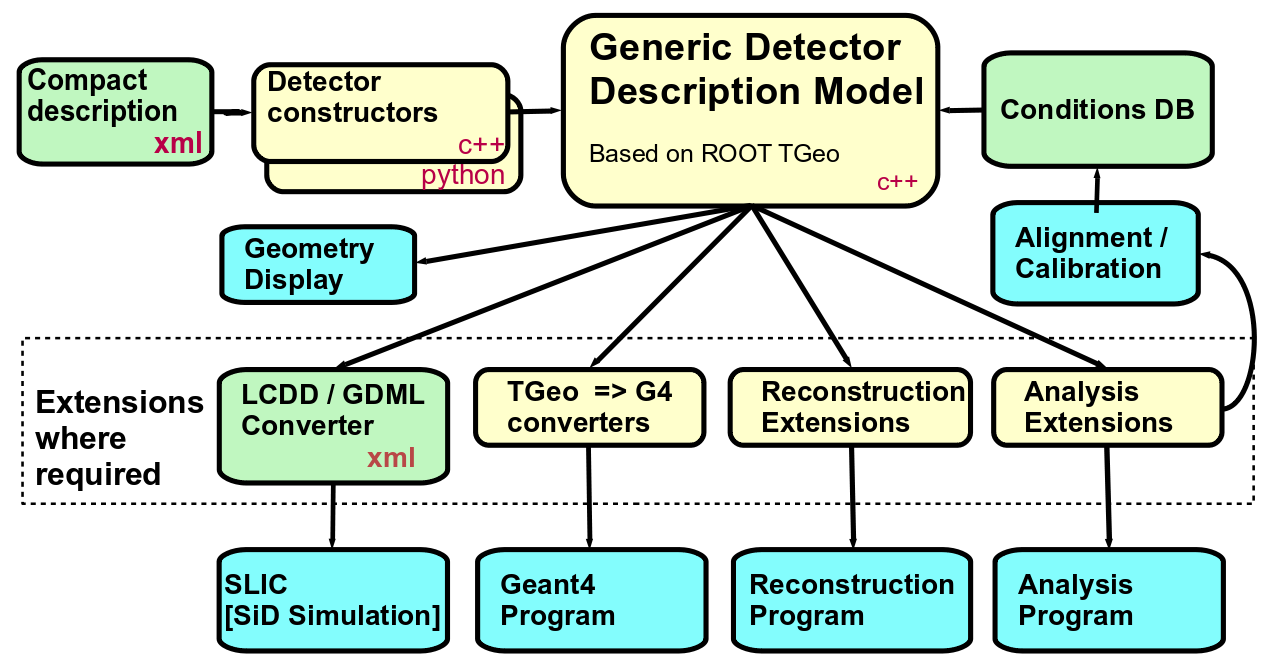
\includegraphics[height=80mm] {DD4hep_big_picture.png}
    \caption{The components of the DD4hep detector geometry toolkit.}
    \label{fig:dd4hep-big-picture}
  \end{center}
  \vspace{-0.4cm}
\end{figure}

%=============================================================================
\subsection{Toolkit Design}
\label{sec:toolkit-design}
%=============================================================================
\noindent
Figure~\ref{fig:dd4hep-big-picture} shows the architecture 
of the main components of the toolkit and their interfaces 
to the end-user applications, namely the simulation, reconstruction, 
alignment and visualization. 
The central element of the toolkit is the so-called generic detector 
description model. This is an in-memory model, i.e., a set of C++ objects 
holding the data describing the geometry and other information of 
the detector. The rest of the toolkit consists of tools and interfaces 
to input or output information from this generic detector model. 
The model and its components will be described in subsequence sections.

%=============================================================================
\subsubsection{The Compact Detector Description}
\label{sec:problem_analysis}
%=============================================================================
\noindent
Inspired from the work of the linear collider detector 
simulation~\cite{bib:LCDD,bib:lcsim}, the compact detector description is used
to define an ideal detector as typically used during 
the conceptual design phase of an experiment. 
The compact description in its minimalistic form is probably not going to 
be adequate later in the detector life cycle and
is likely to be replaced or refined when a more realistic detector 
with deviations from the ideal would be needed by the experiment.

\noindent
In the compact description the detector is parametrized in minimalistic terms
with user provided parameters in XML.
XML is an open format, the DD4hep parsers do not validate against a fix schema
and hence allow to easily introduce new elements and attributes to describe 
detectors. This feature minimizes the burden on the end-user while still 
supporting flexibility.
%Figure~\ref{fig:fig-vxd-xml} shows a partial example of how to describe an ideal 
%silicon-based vertex detector with regular disposition of ladders 
%in 2 layers in total. 
Such a compact detector descriptions cannot be interpreted in a 
general manner, therefore so called $Detector$ $Constructors$ are needed.

%=============================================================================
%\begin{figure}[h]
%  \begin{center}
%    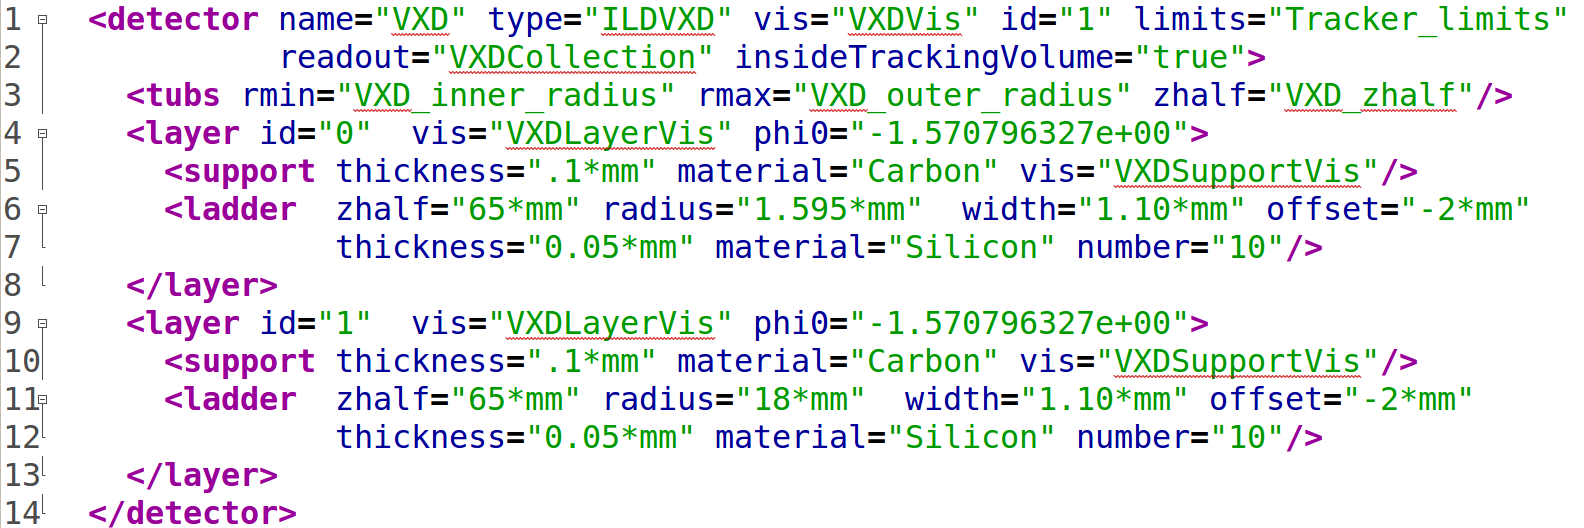
\includegraphics[width=16cm] {DD4hep_compact_xml.png}
%    \caption{An example sniplett of the compact detector description. The 
%             example shows the description of a 2 layered silicon vertex 
%             detector.}
%    \label{fig:fig-vxd-xml}
%  \end{center}
%  \vspace{-0.6cm}
%\end{figure}
%=============================================================================

%=============================================================================
\subsubsection{Detector Constructors}
\label{sec:detector-constructors}
%=============================================================================
\noindent
Detector Constructors are relatively small code fragments that get
as input an XML element from the compact description that represents 
a single detector instance. The code interprets the data and expands 
its geometry model in memory using the elements from the generic detector 
description model described in section~\ref{subsec:generic-model}.
The toolkit invokes these code fragments in a data driven way
using naming conventions during the initialization phase of the 
application. Users focus on one 
single detector type at the time, but the toolkit supports them to still
construct complex and large detector setups. 
Two implementations are currently supported: One is based on 
C++, which performs better and is able to detect errors at 
compiler time, but the code is slightly more technical.
The other is based on Python fragments, the code is more readable and
compact but errors are only detected at execution time.

\noindent
The compact description together with the detector constructors are sufficient
to build the detector model and to visualize it. If during the lifetime of the
experiment the detector model changes, the corresponding constructors will 
need to be adapted accordingly. 
DD4hep provides already a palette of basic pre-implemented geometrical detector 
concepts to design experiments. In view of usage of DD4hep as a detector 
description toolkit, this library may in the future also adopt
generic designs of detector components created by end users e.g. during the design 
phase of future experiments.
%=============================================================================
\begin{figure}[t]
  \begin{center}
    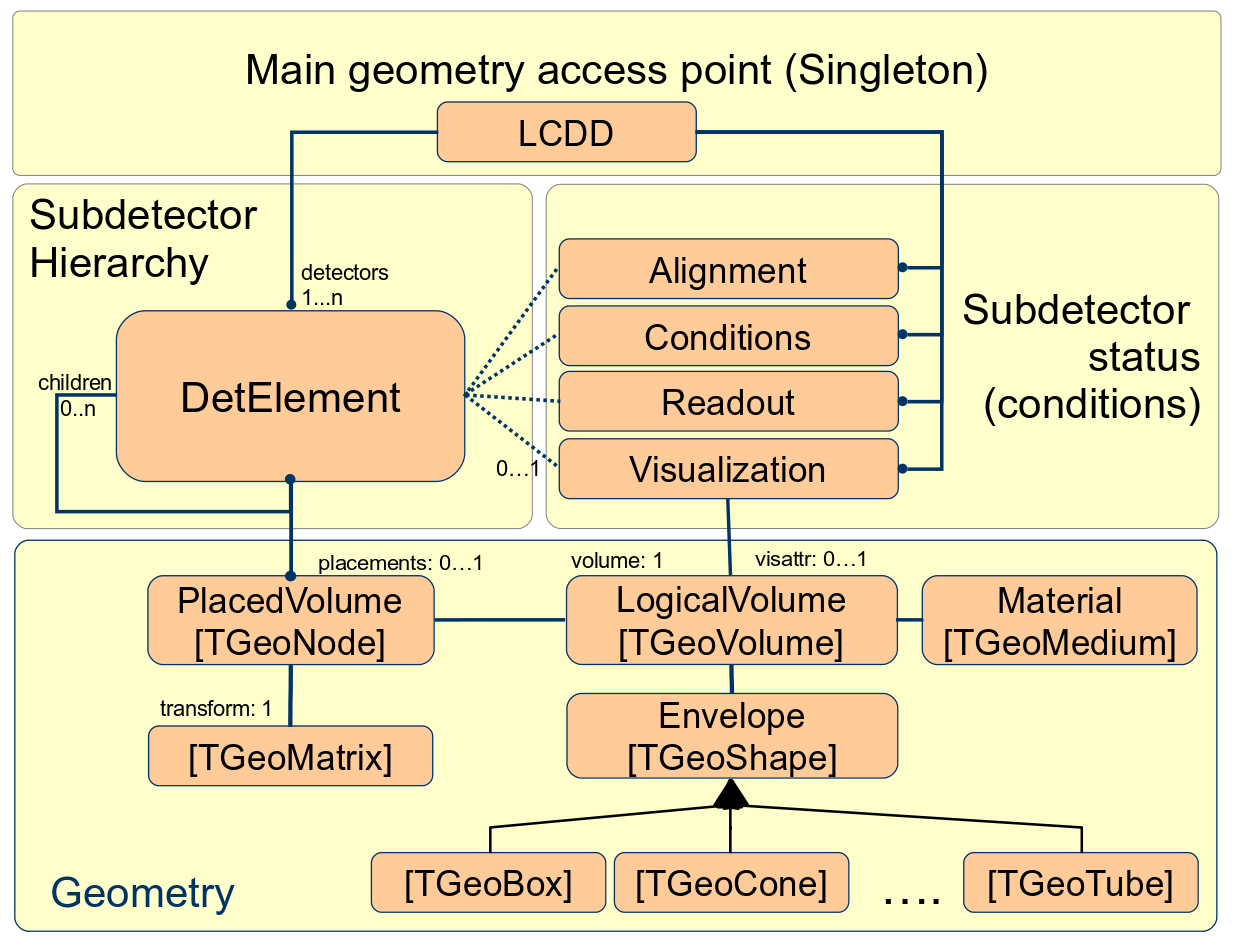
\includegraphics[height=110mm] {DD4hep_classes.png}
    \caption{Class diagram with the main classes and their relations 
             for the Generic Detector Description Model. The implementing
             ROOT classes are shown in brackets.}
    \label{fig:dd4hep-detector-model}
  \end{center}
\end{figure}
%=============================================================================
\subsection{Generic Detector Description Model}
\label{subsec:generic-model}
%=============================================================================

\noindent
This is the heart of the DD4hep detector description toolkit. Its purpose is 
to build in memory a model of the detector including its geometrical aspects
as well as structural and functional aspects. The design reuses the elements 
from the ROOT geometry package and extends them in case required functionality 
is not available. Figure~\ref{fig:dd4hep-detector-model} illustrates the main
players and their relationships.
Any detector is modeled as a tree of $Detector$ $Elements$, the entity 
central to this design, which is represented in the implementation by 
the $DetElement$ class~\cite{bib:LHCb-geometry}. It offers all
applications a natural entry point to any detector part of the experiment
and represents a complete sub-detector (e.g. TPC), a part of a 
sub-detector (e.g. TPC-Endcap), a detector module or any other convenient 
detector device. 
The main purpose is to give access to the data associated 
to the detector device. For example, if the user writes some TPC reconstruction 
code, accessing the TPC detector element from this code will provide access 
the all TPC geometrical dimensions, the alignment and calibration constants 
and other slow varying conditions such as the gas pressure, end-plate 
temperatures etc. The $Detector$ $Element$ acts as a data concentrator. 
Applications may access the full experiment geometry and all connected data
through a singleton object called $LCDD$, which provides 
management, bookkeeping and ownership to the model instances.

\noindent
The geometry is implemented using the ROOT geometry classes, which are used
directly without unnecessary interfaces to isolate the end-user from the 
actual ROOT based implementation. There is one exception: 
The constructors are wrapped to facilitate a very compact and readable 
notation to end-users building custom $Detector$ $Constructors$.

%=============================================================================
\subsubsection{Detector Element Tree versus the Geometry Hierarchy}
\label{subsect:detelement-hierarchy}
%=============================================================================
\noindent
The geometry part of the detector description is delegated to the ROOT classes.
$Logical$ $Volumes$ are the basic objects used in building the geometrical hierarchy. 
A $Logical$ $Volume$ is a shape with its dimensions and consist of a given material. 
They represent unpositioned objects which store all information about 
the placement of possibly embedded volumes. The same
volume can be replicated several times in the geometry. The $Logical$ $Volume$ also 
represents a system of reference with respect to its containing volumes.
The reuse of instances of $Logical$ $Volumes$ for different placements 
optimizes the memory consumption and detailed geometries for complex setups
consisting of millions of volumes may be realized with reasonable amount of memory.
The difficulty is to identify a given positioned volume 
in space and e.g. applying misalignment to one of these volumes. 
The relationship between the Detector Element and the placements
is not defined by a single reference to the placement, but the full path 
from the top of the detector geometry model to resolve existing
ambiguities due to the reuse of $Logical$ $Volumes$.
Hence, individual volumes must be identified by their full path from mother 
to daughter starting from the top-level volume. 

%=============================================================================
\begin{figure}[t]
  \begin{center}
    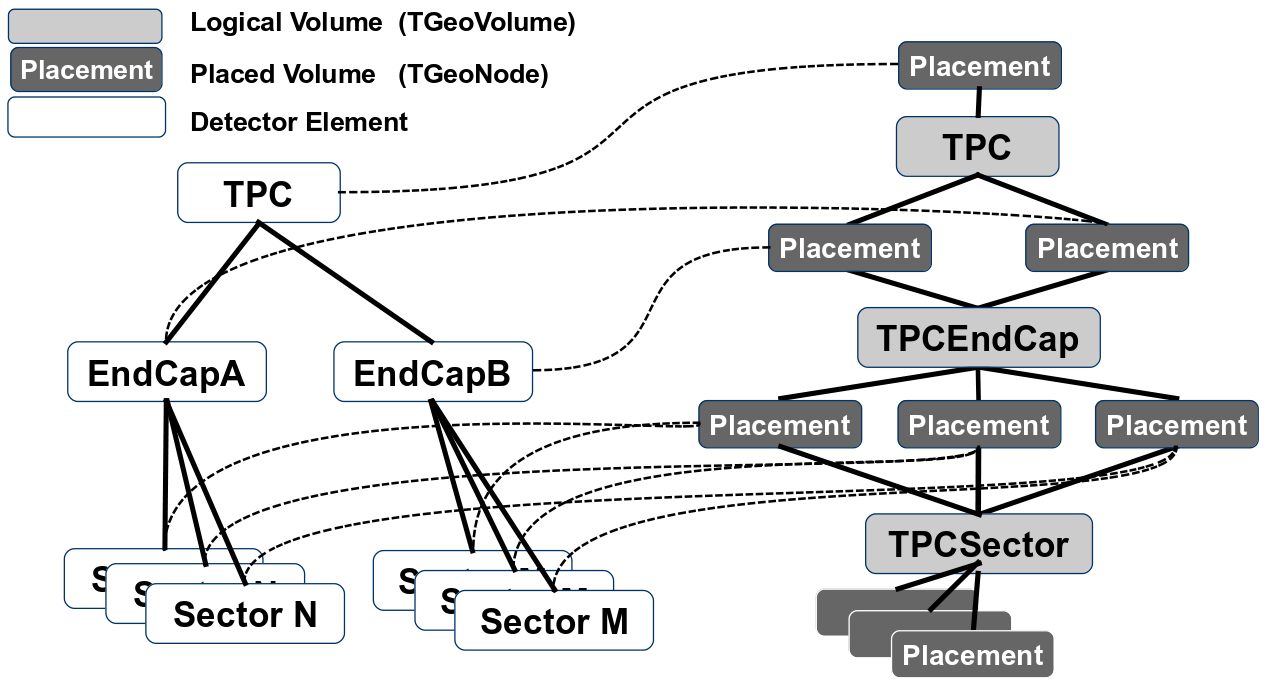
\includegraphics[height=85mm] {DD4hep_detelement_tree.png}
    \caption{The object diagram of a hypothetical TPC detector showing in
    parallel the $Detector$ $Element$ and the $Geometry$ hierarchy and the 
    relationships between the objects.}
    \label{fig:dd4hep-hierarchies}
  \end{center}
\end{figure}
%=============================================================================

\noindent
The tree structure of
Detector Elements is a parallel structure to the geometrical hierarchy.
This structure will probably not be as deep as the geometrical one since 
there would not need to associate detector information at very fine-grain 
level - it is unlikely that every little metallic screw
needs associated detector information such as alignment, conditions, etc.
Though this screw and many other replicas must be described in the geometry 
description since it may be important e.g. for its material contribution 
in the simulation application. Thus, the tree of Detector Elements is
fully degenerate and each detector element object will be placed only 
once in the detector element tree as illustrated for a hypothetical
TPC detector in Figure~\ref{fig:dd4hep-hierarchies}.

%=============================================================================
\subsubsection{Extensions and Views}
\label{subsect:extesions-and-views}
%=============================================================================

\noindent
As depicted in Figure~\ref{fig:dd4hep-big-picture} the reconstruction 
application will require special functionality extending the basics 
offered by the common detector element. This functionality may be
implemented by a set of specialized classes that will extend the 
detector element. These extensions will be in charge 
of providing specific answers to the questions formulated by the 
reconstruction algorithms such as pattern recognition, tracking, vertexing, 
particle identification, etc. One example could be to transform a calorimeter 
cell identifier into a 3D space position in the global coordinate system.
A generic detector description toolkit would be unable 
to answer this concrete question, however it provides a convenient 
environment for the developer to slot-in code fragments, which implement the
additional functionality using parameters stored
in the XML compact description.

\noindent
Depending on the functionality these specialized component must be able to
either store additional data, expose additional behavior or both. Additional 
behavior may easily be added overloading the $DetElement$ class using its 
internal data. The internal data is public and addressed by reference, hence
any number of views extending the $DetElement$ behavior may be constructed 
with very small overhead. Additional data may be added by any user at any time
to any instance of the $DetElement$ class using a simple aggregation 
mechanism shown in Figure~\ref{fig:dd4hep-extensions}. Data extensions must 
differ by their type. The freedom to attach virtually
any data item allows for optimized attachments depending on the 
application type, such as special attachments for reconstruction, 
simulation, tracking, etc.
%=============================================================================
\begin{figure}[t]
  \begin{center}
    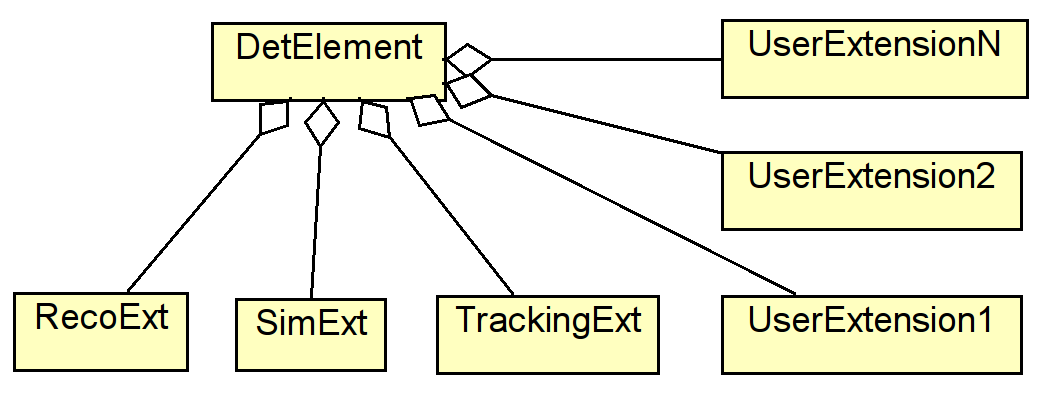
\includegraphics[width=115mm] {DD4hep-extensions.png}
    \caption{Extensions may be attached to common Detector Elements which 
             extend the functionality of the common DetElement 
             class and support e.g. caching of precomputed values.}
    \label{fig:dd4hep-extensions}
  \end{center}
\end{figure}
%=============================================================================
This design allows to build views addressing the following use-cases:
\begin{itemize}
\item{{\bf{Convenience Views}}} provide higher level abstractions
    and internally group complex calculations. Such views simplify 
    the life of the end-users.
\item{{\bf{Optimization Views}}} allows end-users extend the data of 
    the common detector detector element and store precomputed 
    results, which would be expensive to obtain repeatedly.
\item{{\bf{Compatibility Views}}} help to ensure smooth periods of 
    software redesign. During the life-time of the experiment
    often various software constructs are for functional reasons 
    re-designed and re-engineered.
    Compatibility Views either adapt new data designs to existing application 
    code or expose new behavior based on existing data.
\end{itemize}

%=============================================================================
\subsection{Simulation Support}
\label{subsect:simulation-support}
%=============================================================================
\noindent
Detector-simulation depends strongly on the use of an underlying simulation toolkit, 
the most prominent candidate nowadays being Geant4~\cite{bib:geant4}.
DD4hep supports simulation activities with Geant4 providing
an automatic translation mechanism between geometry representations.
The simulation response in the active elements of the detector
is not implemented by the toolkit, since it is strongly influenced by the technical 
choices and precise simulations depends on the very specific detection techniques.
In Geant4 this response is computed in software constructs called $Sensitive$ 
$Detectors$.

\noindent
Ideally DD4hep aims to provide a generic simulation application.
Similar to the palette of pre-implemented geometrical detector 
concepts to design experiments, it provides a palette of $Sensitive$
$Detectors$ to simulate the detector response in form of a component library.
Detector designers may base the simulation of a planned experiment 
on these predefined components for initial design and optimization 
studies.  In a similar way easy access
and configuration of other user actions of Geant4 is provided.

%=============================================================================
\subsection{Detector Alignment Support}
\label{subsect:alignment-support}
%=============================================================================
\noindent
The support for alignment operations is crucial to the usefulness of the
toolkit. In the linear collider community this support is basically missing 
in all the currently used geometry description systems.
The possibility to apply into the detector description alignment $deltas$ 
(differences with respect the ideal or measured position) and read them 
from an external source is mandatory to exploit the toolkit. A typical 
alignment application would consist of calculating a new set of $deltas$
from a given starting point, which could then be loaded and applied again 
in order to validate the alignment by recalculating some alignment residuals.
The ROOT geometry package supports to apply an [mis]-alignment to 
$touchable$ objects in the geometry. $Touchable$ objects are identified 
by the path of positioned volumes starting with the top node 
(e.g. path=$/TOP/A_1/B_4/C_3$). Contrary to ordinary multiple placements
of $Logical$ $Volumes$, $touchable$ objects are degenerate and only 
valid for one single volume~\cite{bib:ROOT-tgeo}. 
To simplify the usage for the end user,
the identification of a positioned volume will be connected
to the Detector Element, where only the relative path with respect 
to the Detector Element will have to be specified 
rather the full path from the top volume.
The $delta$-values will have to be read from various data sources.
The initial implementation will be based on simple XML files, later
a connection to other sources such as the detector conditions database
is envisaged.



\noindent
The alignment support will be subject to a separate development line of the
\DDhep toolkit, called \DDA and hence will be discussed in another 
manual~\cite{bib:DDAlign}.
%
\newpage
%=============================================================================
% Manual
%=============================================================================
\section{User Manual}
\label{sec:dd4hep-user-manual}
%=============================================================================
\noindent
This chapter describes how supply a physics application developed with all the 
information related to the detector which is necessary to process data from 
particle collisions and to qualify the detecting apparatus in order to 
interpret these event data.

\noindent
The clients of the detector description are the algorithms residing in the 
event processing framework that need this information in order to perform 
their job (reconstruction, simulation, etc.). 
The detector description provided by \DDhep is a framework for developers 
to provide the specific detector information to software algorithms, which 
process data from particle collisions.

\noindent
In the following sections an overview is given over the various independent
elements of \DDhep followed by the discussion of an example which leads to 
the description of a detector when combining these elements.
This includes a discussion of the features of the \DDhep detector description
and of its structure. 

%=============================================================================
\subsection{Building DD4hep}
\label{sec:dd4hep-user-manual-building}
%=============================================================================

\noindent
The \DDhep source code is freely available. See the 
\detdesc{doc/LICENSE}{licence conditions}.
Please read the \detdesc{doc/release.notes}{Release Notes} 
before downloading or using this release.

\noindent
The \DDhep project consists of several packages. The idea 
has been to separate the common parts of 
the detector description toolkit from concrete detector examples. 

\noindent
The package {\tw{DDCore}} contains the definition of the basic classes 
of the toolkit: \tw{Handle}, \tw{DetElement}, \tw{Volume}, \tw{PlacedVolume},
\tw{Shapes}, \tw{Material}, etc. Most of these classes are \tw{handles} 
to ROOT's TGeom classes.

%=============================================================================
\subsubsection{Supported Platforms}
\label{sec:dd4hep-user-manual-platforms}
%=============================================================================
\noindent
Supported platforms for DD4hep are the CERN Linux operating systems:
\begin{itemize}
\item \tw{Scientic} \tw{Linux} \tw{CERN} \tw{6}
\item \tw{Scientic} \tw{Linux} \tw{CERN} \tw{7} - once approved.
\end{itemize}
Support for any other platform will well be taken into account, but can only
be actively supported by users who submit the necessary patches.

%=============================================================================
\subsubsection{Prerequisites}
\label{sec:dd4hep-user-manual-prerequisites}
%=============================================================================
\noindent
DD4hep depends on a number of $external$ packages. 
The user will need to install these in his/her 
system before building and running the examples
\begin{itemize}\itemcompact
\item Mandatory are recent \tw{CMake} (version 2.8 or higher) and 
\item \tw{ROOT} (version 5.34 or higher) installations.~\footnote{Please 
not, that due to the removal of the Reflex plugin mechanism from ROOT 6,
version 6 of ROOT is currently not supported. This deficiency will be waved 
in the future.}
\item If the \tw{Xerces-C} is used to parse compact descriptions and 
        installation of {Xerces-C} will be required.
\item To build \DDG it is mandatory to have an installation of the Boost
    header files.
\item To build and run the simulation examples \tw{Geant4} will be required. 
\end{itemize}

\newpage
%=============================================================================
\subsubsection{CMake Build Options for DD4hep}
\label{sec:dd4hep-user-manual-building}
%=============================================================================
\noindent
The package provides the basic mechanisms for constructing the 
{\it{Generic Detector Description Model}} in memory from XML compact detector 
definition files. Two methods are currently supported: one based
on the C++ \tw{Xerces}-C parser, and another one based on Python and using the 
\tw{PyROOT} bindings to ROOT~\footnote{I will not continue 
the support using PyROOT. \\
If there is a desire that it stays alive 
someone else should take care -- M.Frank}. 
\tw{PyROOT} may be enabled using the switch:

\begin{unnumberedcode}
    -DD4HEP_USE_PYROOT:BOOL
\end{unnumberedcode}

\noindent
The XML parsing method is enabled by default using the \tw{TiXML} parser. Optionally 
instead of \tw{TiXML} the \tw{Xerces}-C  parser may be chosen by setting the 
two configuration options appropriately:

\begin{unnumberedcode}
    -DD4HEP_USE_XERCESC:BOOL
    -DXERCESC_ROOT_DIR=<path to Xerces-C-installation-directory>
\end{unnumberedcode}

\noindent
{\bf{DDG4}} is the package that contains the conversion of \DDhep geometry 
into Geant4 geometry to be used for simulation. 
The option \tw{DD4HEP\_WITH\_GEANT4:BOOL} controls the building or not of 
this package that has the dependency to Geant4. The Geant4 installation 
needs to be located using the variable:

\begin{unnumberedcode}
   -DDD4HEP_WITH_GEANT4=on -D 
   -DGeant4_DIR=<path to Geant4Config.cmake>
\end{unnumberedcode}

\noindent
To properly handle component properties using \tw{boost::spirit}, 
access to the Boost header files must be provided.
\vspace{0.3cm}
\begin{unnumberedcode}
    -DDD4HEP_USE_BOOST=ON 
    -DBOOST_INCLUDE_DIR=<path to the boost include directory>
\end{unnumberedcode}

\noindent
Other useful build options:
\begin{itemize}
\item build doxygen documentation ( after 'install' open ./doc/html/index.html)
\begin{unnumberedcode}
    -D INSTALL_DOC=on 
\end{unnumberedcode}
 
\item {\bf{note:}} you might have to update your environment beforehand to have all needed 
     libraries in the shared lib search path (this will vary with OS, shell, etc.) e.g 
\begin{unnumberedcode}
      . /data/ilcsoft/geant4/9.5/bin/geant4.sh
      export CLHEP_BASE_DIR="/data/ilcsoft/HEAD/CLHEP/2.1.0.1"
      export CLHEP_INCLUDE_DIR="$CLHEP_BASE_DIR/include"
      export PATH="$CLHEP_BASE_DIR/bin:$PATH"
      export LD_LIBRARY_PATH="$CLHEP_BASE_DIR/lib:$LD_LIBRARY_PATH"
\end{unnumberedcode}
\end{itemize}

%=============================================================================
\subsubsection{Build From Source}
\label{sec:dd4hep-user-manual-building-from-source}
%=============================================================================
\noindent
The following steps are necessary to build \DDhep:
\begin{itemize}
\item Set the environment, at least ROOT needs to be initialized, e.g.
    \begin{unnumberedcode}
      source  /data/ilcsoft/root/5.34.03/bin/thisroot.sh
    \end{unnumberedcode}
    \vspace{-0.6cm}
   (the bare minimum is: \tw{export ROOTSYS=<path to root installation>}).

\item First checkout code from the repository:
    \begin{unnumberedcode}
      svn co https://svnsrv.desy.de/public/aidasoft/DD4hep/trunk DD4hep
    \end{unnumberedcode}
    \vspace{-0.6cm}

\item We refer to the directory \DDhep as the source directory. The 
next step is to create a directory in which to configure and run the build 
and store the build products. This directory should not be the same as, or 
inside, the source directory. In this guide, we create this build directory 
alongside our source directory: 
    \begin{unnumberedcode}
      mkdir build
      cd build
      cmake -DCMAKE_INSTALL_PREFIX=<dd4hep-install-pasth> <CMake-options> ../DD4hep
      make -j 4
      make install
    \end{unnumberedcode}
\end{itemize}
The CMake Variable \tw{CMAKE\_INSTALL\_PREFIX} is used to set the install directory, 
the directory under which the \DDhep libraries, headers and support files 
will be installed.

%=============================================================================
\subsubsection{Tutorial}
\label{sec:dd4hep-user-manual-tutorial}
%=============================================================================
\noindent
In January 2013 an introductory tutorial was given at CERN to members of the 
linear collider community. The slides to the tutorial can be found 
\detdesc{doc/DD4hep_Tutorial.pdf}{here}.
The tutorial is not entirely up to date. Please take the content with a 
grain of salt.

%=============================================================================
\subsubsection{Doxygen Code Documentation}
\label{sec:dd4hep-user-manual-doxygen}
%=============================================================================
\noindent
The \DDhep source code is instrumented with tags understood by doxygen.
The generated code documentation can be found
\detdesc{html/index.html}{here}.

%=============================================================================
\subsubsection{Remarks}
\label{sec:dd4hep-user-manual-remarks}
%=============================================================================
\noindent
The main reference is the doxygen information of \DDhep and the ROOT documentation. 
Please refer to these sources for a detailed view of the capabilities of 
each component and/or its handle.
For coherence reasons, the description of the
interfaces is limited to examples which illustrate the usage of the basic 
components. 

%=============================================================================
\subsubsection{Caveat}
\label{sec:dd4hep-user-manual-caveat}
%=============================================================================
\noindent
The atomic units in of Geant4 are (millimeter, nanosecond and MeV and radians).
The atomic units of ROOT-TGeo are (centimeter, seconds, GeV and degrees).
Unfortunately the authors could not agree on a common system of units
and mixing the two can easily result in a chaos.
Users must be aware of this fact.


\newpage
%=============================================================================
\subsection{DD4hep Handles}
\label{sec:dd4hep-user-manual-handles}
%=============================================================================
\noindent
Handles are the means of clients accessing \DDhep detector description data.
The data itself is not held by the handle itself, the handle only allows the
access to the data typically held by a pointer. The template handle class
(see for details the \detdesc{html/struct_d_d4hep_1_1_geometry_1_1_handle.html}{header file}).
allows type safe assignment of other unrelated handles and supports standard 
data conversions to the underlying object in form of the raw pointer, 
a reference etc. The template handle class:

\begin{code}
template <typename T> class Handle  {
public:
      // Type definitions and class specific abbreviations and forward declarations
      typedef T Implementation;
      typedef Handle<Implementation> handle_t;
public:
      // Single and only data member: pointer to the underlying object  
      T* m_element;

public:
      Handle() : m_element(0)                  {                                     }
      Handle(T* e) : m_element(e)              {                                     }
      Handle(const Handle<T>& e) : m_element(e.m_element) {                          }
      template<typename Q> Handle(Q* e)
      : m_element((T*)e)                       { verifyObject();                     }
      template<typename Q> Handle(const Handle<Q>& e) 
      : m_element((T*)e.m_element)             { verifyObject();                     }
      Handle<T>& operator=(const Handle<T>& e) { m_element=e.m_element; return *this;}
      bool isValid() const                     { return 0 != m_element;              }
      bool operator!() const                   { return 0 == m_element;              }
      void clear()                             { m_element = 0;                      }
      T* operator->() const                    { return  m_element;                  }
      operator T& ()  const                    { return *m_element;                  }
      T& operator*()  const                    { return *m_element;                  }
      T* ptr() const                           { return  m_element;                  }
      template <typename Q> Q* _ptr() const    { return  (Q*)m_element;              }
      template <typename Q> Q*  data() const   { return  (Q*)m_element;              }
      template <typename Q> Q&  object() const { return *(Q*)m_element;              }
      const char* name() const;
};
\end{code}

\noindent
effectively works like a pointer with additional object validation during assignment
and construction. Handles support direct access to the held object: either by using 
the 

\begin{verbatim}
       operator->()                        (See line 16 above)
\end{verbatim}

\noindent
or the automatic type conversions:

\begin{verbatim}
      operator T& ()  const                (See line 17-18 above)
      T& operator*()  const.
\end{verbatim}

\noindent
All entities of the \DDhep detector description are exposed as handles - 
raw pointers should not occur in the code. 
The handles to these objects serve two purposes:
\begin{itemize}\itemcompact
\item Hold a pointer to the object and extend the functionality of a raw
    pointer.
\item Enable the creation of new objects using specialized constructors
    within sub-classes. To ensure memory integrity and avoid resource 
    leaks these created objects should always be stored in the 
    detector description data hub $LCDD$ described in 
    section~\ref{sec:dd4hep-user-manual-LCDD-hub}.
\end{itemize}

\newpage
%=============================================================================
\subsection{The Data Extension Mechanism}
\label{sec:dd4hep-user-manual-data-extensions}
%=============================================================================
\noindent
Data extensions are client defined C++ objects aggregated to basic \DDhep objects.
The need to introduce such data extensions results from the simple fact that
no data structure can be defined without the iterative need in the long term
to extend it leading to implementations, which can only satisfy a subset of 
possible clients. To accomplish for this fact a mechanism was put in place
which allows any user to attach any supplementary information provided
the information is embedded in a polymorph object with an accessible destructor.
There is one limitation though: object extension must differ by their 
interface type. 
There may not be two objects attached with the identical interface type.
The actual implemented sub-type of the extension is not relevant.
Separating the interface type from the implementation type keeps client
code still functional even if the implementation of the extension changes 
or is a plug-able component.

\noindent
The following code snippet shows the extension interface:

\begin{code}
  /// Extend the object with an arbitrary structure accessible by the type
  template <typename IFACE, typename CONCRETE> IFACE* addExtension(CONCRETE* c);
  /// Access extension element by the type
  template <class T> T* extension() const;
\end{code}

Assuming a client class of the following structure:
\begin{code}
    class ExtensionInterface {
      virtual ~ExtensionInterface();
      virtual void foo() = 0;
    };

    class ExtensionImplementation : public ExtensionInterface {
      ExtensionImplementation();
      virtual ~ExtensionImplementation();
      virtual void foo();
    };
\end{code}
is then attached to an extensible object as follows:
\begin{code}
    ExtensionImplementation* ptr = new ExtensionImplementation();
    ... fill the ExtensionImplementation instance with data ...
    module.addExtension<ExtensionInterface>(ptr);
\end{code}
The data extension may then be retrieved whenever the instance of the
extensible object "module" is accessible:
\begin{code}
    ExtensionInterface* ptr = module.extension<ExtensionInterface>();
\end{code}
The lookup mechanism is rather efficient. Though it is advisable to
cache the pointer withing the client code if the usage is very frequent.


\noindent
There are currently three object types present which support this mechanism:
\begin{itemize}\itemcompact
\item the central object of \DDhep, the \tw{LCDD} class discussed in 
        section~\ref{sec:dd4hep-user-manual-LCDD-hub}.
\item the object describing subdetectors or parts thereof, the 
        \tw{DetElement} class discussed in 
        section~\ref{sec:dd4hep-user-manual-detector-elements}.
        Detector element extensions in addition require the presence 
        of a copy constructor to support e.g. reflection operations.
        Without a copy mechanism detector element hierarchies could 
        cloned.
\item the object describing sensitive detectors, 
       the \tw{SensitiveDetector} class discussed in 
       section~\ref{sec:dd4hep-user-manual-sensitive-detectors}.
\end{itemize}


\newpage
%=============================================================================
\subsection{XML Tools and Interfaces}
\label{sec:dd4hep-user-manual-xml-tools}
%=============================================================================
\noindent
Using native tools to interpret XML structures is rather tedious and lengthy.
To easy the access to XML data considerable effort was put in place to easy
the life of clients as much as possible using predefined constructs to 
access XML attributes, elements or element collections.

\noindent 
The functionality of the XML tools is perhaps best shown with a small example.
Imagine to extract the data from an XML snippet like the following:
\begin{code}
  <detector name="Sometthing">
    <tubs rmin="BP_radius - BP_thickness" rmax="BP_radius" zhalf="Endcap_zmax/2.0"/>
    <position x="0" y="0" z="Endcap_zmax/2.0" />
    <rotation x="0.0" y="CrossingAngle/2.0" z="0.0" />
    <layer id="1" inner_r="Barrel_r1" 
    	   outer_r="Barrel_r1 + 0.02*cm" inner_z="Barrel_zmax + 0.1*cm">
      <slice material = "G10" thickness ="0.5*cm"/>
    </layer>
    <layer id="2" inner_r="Barrel_r2" 
	   outer_r="Barrel_r2 + 0.02*cm" inner_z="Barrel_zmax + 0.1*cm">
     <slice material = "G10" thickness ="0.5*cm"/>
    </layer>
    ....
  </detector>
\end{code}

The variable names used in the XML snippet are evaluated when interpreted.
Unless the attributes are accessed as strings, the client never sees the 
strings, but only the evaluated numbers.
The anatomy of the C++ code snippets to interpret such a data section 
looks very similar:
\begin{code}
  static void some_xml_handler(xml_h e)  {
    xml_det_t  x_det  (e);
    xml_comp_t x_tube    = x_det.tubs();
    xml_dim_t  pos       = x_det.position();
    xml_dim_t  rot       = x_det.rotation();
    string     name      = x_det.nameStr();
      
    for(xml_coll_t i(x_det,_U(layer)); i; ++i)  {
      xml_comp_t x_layer = i;
      double  zmin = x_layer.inner_z();
      double  rmin = x_layer.inner_r();
      double  rmax = x_layer.outer_r();
      double  layerWidh = 0;
        
      for(xml_coll_t j(x_layer,_U(slice)); j; ++j)  {
        double thickness = xml_comp_t(j).thickness();
        layerWidth += thickness;
      }
    }
  }
\end{code}
In the above code snippet an XML (sub-)tree is passed to the executing 
function as a handle to an XML element ({\tt{xml\_h}}). Such handles may seamlessly be
assigned to any supporting helper class inheriting from the
class {\tt{XML::Element}}, which encapsulates the functionality required to 
interpret the XML structures.
Effectively the various XML attributes and child nodes 
are accessed using functions with the same
name from a convenience handle. 
In lines 3-5 child nodes are extracted, lines 10-12,16 access element attributes.
Element collections with the same tag names \tw{layer} and \tw{slice} are exposed
to the client code using an iteration mechanism.

\noindent
Note the macros $\tt{\_U(layer)}$ and $\tt{\_U(slice)}$: 
When using Xerces-C as an XML parser, 
it will expand to the reference to an object containing the unicode value 
of the string "layer". The full list of predefined tag names can be found in the
include file \detdesc{html/_unicode_values_8h.html}{DD4hep/UnicodeValues.h}.
If a user tag is not part in the precompiled tag list, the corresponding Unicode
string may be created with the macro \tw{\_Unicode(layer)} or the function
\tw{Unicode("layer")}.

\noindent
The convenience handles actually implement
these functions to ease life. There is no magic - newly created attributes
with new names obviously cannot be accessed with convenience mechanism.
Hence, either you know what you are doing and you create your own 
convenience handlers or you restrict yourself a bit in the creativity
of defining new attribute names.

\noindent
There exist several utility classes to extract data from predefined XML tags:
\begin{itemize}\itemcompact
\item Any XML element is described by an XML handle
       \detdesc{html/struct_d_d4hep_1_1_geometry_1_1_handle.html}{\tt{XML::Handle\_t}} 
       ({\tt{xml\_t}}). Handles are the basic structure for the support
       of higher level interfaces described above. The assignment of a handle
       to any of the interfaces below is possible.
\item The class \detdesc{html/struct_d_d4hep_1_1_x_m_l_1_1_element.html}{\tt{XML::Element}} 
       ({\tt{xml\_elt\_t}})
       supports in a simple way the navigation through the hierarchy of the 
       XML tree accessing child nodes and attributes. Attributes at this
       level are named entities and the tag name must be supplied.
\item The class \detdesc{html/struct_d_d4hep_1_1_x_m_l_1_1_dimension.html}{\tt{XML::Dimension}} 
       with the type definition {\tt{xml\_dim\_t}}, 
       supports numerous access functions named identical to the
       XML attribute names. Such helper classes simplify the tedious
       string handling required by the 
\item The class \detdesc{html/struct_d_d4hep_1_1_x_m_l_1_1_component.html}{\tt{XML::Component}} 
       ({\tt{xml\_comp\_t}}) and \\
       the class \detdesc{html/struct_d_d4hep_1_1_x_m_l_1_1_det_element.html}{\tt{XML::Detector}}
       ({\tt{xml\_det\_t}}) resolving other issues useful to construct detectors.
\item Sequences of XML elements with an identical tag name may be handled
       as iterations as shown in the Figure above using the class
       \detdesc{html/struct_d_d4hep_1_1_x_m_l_1_1_collection__t.html}{\tt{XML::Collection\_t}}.
\item Convenience classes, which allow easy access to element attributes 
       may easily be constructed using the methods of the {\tt{XML::Element}}
       class. This allows to construct very flexible thou non-intrusive 
       extensions to \DDhep. Hence there is a priori no need to modify
       these helpers for the benefit of only one single client.
       In the presence of multiple requests such extensions may though be adopted.
\end{itemize}
It is clearly the responsibility of the client to only request attributes
from an XML element, which exist. If an attribute, a child node etc. is not 
found within the element an exception is thrown.

\noindent
The basic interface of the \tw{XML::Element} class allows to access tags
and child nodes not exposed by the convenience wrappers:
\begin{code}
  /// Access the tag name of this DOM element
  std::string tag() const;
  /// Access the tag name of this DOM element
  const XmlChar* tagName() const;

  /// Check for the existence of a named attribute
  bool hasAttr(const XmlChar* name) const;
  /// Retrieve a collection of all attributes of this DOM element
  std::vector<Attribute> attributes() const;
  /// Access single attribute by it's name
  Attribute getAttr(const XmlChar* name) const;
  /// Access attribute with implicit return type conversion
  template <class T> T attr(const XmlChar* tag) const;
  /// Access attribute name (throws exception if not present)
  const XmlChar* attr_name(const Attribute attr) const;
  /// Access attribute value by the attribute  (throws exception if not present)
  const XmlChar* attr_value(const Attribute attr) const;

  /// Check the existence of a child with a given tag name
  bool hasChild(const XmlChar* tag) const;
  /// Access child by tag name. Thow an exception if required in case the child is not present
  Handle_t child(const Strng_t& tag, bool except = true) const;
  /// Add a new child to the DOM node
  Handle_t addChild(const XmlChar* tag) const;
  /// Check if a child with the required tag exists - if not create it and add it to the current node
  Handle_t setChild(const XmlChar* tag) const;
\end{code}

%=============================================================================
\subsection{The Detector Description Data Hub: LCDD}
\label{sec:dd4hep-user-manual-LCDD-hub}
%=============================================================================
\noindent
As shown in Figure~\ref{fig:dd4hep-detector-model}, any access to the detector 
description data is done using a standardized interface called \tw{LCDD}.
During the configuration phase of the detector the interface is used to populate
the internal data structures.
Data structures present in the memory layout of the detector description
may be retrieved by clients at any time using the 
\detdesc{html/struct_d_d4hep_1_1_geometry_1_1_l_c_d_d.html}{\tw{LCDD} interface class}.
This includes of course, the access during the actual detector construction.
The following code listing shows the accessor method to retrieve 
detector description entities from the interface. Not shown are access methods
for groups of these entities and the methods to add objects:

\begin{code}
struct LCDD {

  ///+++ Shortcuts to access often used quantities

  /// Return handle to material describing air
  virtual Material air() const = 0;
  /// Return handle to material describing vacuum
  virtual Material vacuum() const = 0;
  /// Return handle to "invisible" visualization attributes
  virtual VisAttr  invisible() const = 0;

  ///+++ Access to the top level detector elements and the corresponding volumes

  /// Return reference to the top-most (world) detector element
  virtual DetElement    world() const = 0;
  /// Return reference to detector element with all tracker devices.
  virtual DetElement    trackers() const = 0;

  /// Return handle to the world volume containing everything
  virtual Volume        worldVolume() const = 0;
  /// Return handle to the volume containing the tracking devices
  virtual Volume        trackingVolume() const = 0;

  ///+++ Access to geometry and detector description objects

  /// Retrieve a constant by it's name from the detector description
  virtual Constant      constant(const std::string& name)      const = 0;
  /// Retrieve a matrial by it's name from the detector description
  virtual Material      material(const std::string& name)      const = 0;
  /// Retrieve a field component by it's name from the detector description
  virtual DetElement    detector(const std::string& name)      const = 0;
  /// Retrieve a sensitive detector by it's name from the detector description
  virtual SensitiveDetector sensitiveDetector(const std::string& name) const = 0;
  /// Retrieve a readout object by it's name from the detector description
  virtual Readout       readout(const std::string& name)       const = 0;
  /// Retrieve a id descriptor by it's name from the detector description
  virtual IDDescriptor  idSpecification(const std::string& name)   const = 0;
  /// Retrieve a subdetector element by it's name from the detector description
  virtual CartesianFieldfield(const std::string& name)     const = 0;

  ///+++ Access to visualisation attributes and Geant4 processing hints

  /// Retrieve a visualization attribute by it's name from the detector description
  virtual VisAttr       visAttributes(const std::string& name) const = 0;

  /// Retrieve a region object by it's name from the detector description
  virtual Region        region(const std::string& name)    const = 0;
  /// Retrieve a limitset by it's name from the detector description
  virtual LimitSet      limitSet(const std::string& name)      const = 0;
  /// Retrieve an alignment entry by it's name from the detector description
  virtual AlignmentEntryalignment(const std::string& path)     const = 0;
  ...
  
  ///+++ Extension mechanism:

  /// Extend the sensitive detector element with an arbitrary structure accessible by the type
  template <typename IFACE, typename CONCRETE> IFACE* addExtension(CONCRETE* c);
  /// Access extension element by the type
  template <class T> T* extension() const;
};
\end{code}

\noindent
As shown in the above listing, the \tw{LCDD} interface is the main access point to access
a whole set 
\begin{itemize}\itemcompact
\item often used predefined values such as the material "air" or "vacuum" (line 5-10).
\item the top level objects "world", "trackers" and the corresponding volumes (line 14-22).
\item items in the constants table containing named definitions also used during the
  interpretation of the XML content after parsing (line 27)
\item named items in the the material table (line 29)
\item named subdetectors after construction and the corresponding (line 31)
\item named sensitive detectors with their (line 33)
\item named readout structure definition using a (line 35)
\item named readout identifier descriptions (line 37)
\item named descriptors of electric and/or magnetic fields  (line 39).
\end{itemize}
Additional support for specialized applications is provided by the interface:
\begin{itemize}\itemcompact
\item Geant4: named region settings  (line 47)
\item Geant4: named limits settings  (line 49)
\item Visualization: named visualization attributes  (line 44)
\item Alignment: named alignment entries to correct displaced volumes  (line 51)
\item User defined extensions (line 56-59) are supported with the extension mechanism 
    described in section~\ref{sec:dd4hep-user-manual-data-extensions}.
\end{itemize}
All the values are populated either directly from XML or from
\tw{detector-constructors} (see section~\ref{sec:detector-constructors}). The interface
also allows to load XML configuration files of any kind provided an appropriate 
interpretation plugin is present. In the next section we describe the functionality 
of the "lccdd" plugin used to interpret the compact detector description.
This mechanism can easily be extended using ROOT plugins, where the 
plugin name must corrspond to the XML root element of the document to 
be interpreted.

\newpage
%=============================================================================
\subsection{Detector Description Persistency in XML}
\label{sec:compact-xml-structure}
%=============================================================================
\noindent
As explained in a previous section, the mechanism involved in the data loading 
allow an application to be fairly independent of the technology used to populate
the transient detector representation. However, if one wants to use a given tech-
nology, she/he has to get/provide the corresponding conversion mechanism.
Though \DDhep also supports the population of the detector description using 
python constructs, we want to focus here on the XML based population.
The choice of XML was driven mainly by its easiness of use and the number 
of tools provided for its manipulation and parsing. Moreover, XML data
can be easily translated into many other format using tools like \tw{XSLT} 
processors.
The grammar used for the XML data is pretty simple and straight forward, 
actually very similar to other geometry description languages based
on XML. For example the material description is nearly identical
to the material description in \tw{GDML}~\cite{bib:GDML}.
The syntactic structure of the compact XML description was taken from
the SiD detector description~\cite{bib:LCDD}.
The following listing shows the basic layout of any
the compact detector description file with its different sections:

\begin{code}
<lccdd>
    <info>          ...    </info>             Auxiliary detector model information
    <includes>      ...    </includes>         Section defining GDML files to be included
    <define>        ...    </define>           Dictionary of constant expressions and varables
    <materials>     ...    </materials>        Additional material definitions
    <display>       ...    </display>          Definition of visualization attributes
    <detectors>     ...    </detectors>        Section with sub-detector definitions
    <readouts>      ...    </readouts>         Section with readout structure definitions
    <limits>        ...    </limits>           Definition of limit sets for Geant4
    <fields>        ...    </fields>           Field definitions
</lccdd>
\end{code}

\noindent
The root tag of the XML tree is {\tw{lccdd}}. This name is fixed.
In the following the content of the various sections is discussed.
The XML sections are filled with the following information:
\begin{itemize}
\item {\bf{The \tw{<info>} sub-tree}} contains auxiliary information about 
       the detector model:

\begin{code}
<info name="clic_sid_cdr"
      title="CLIC Silicon Detector CDR"
      author="Christian Grefe"
      url="https://twiki.cern.ch/twiki/bin/view/CLIC/ClicSidCdr"
      status="development"
      version="$Id: compact.xml 665 2013-07-02 18:49:26Z markus.frank $">
      <comment>The compact format for the CLIC Silicon Detector used 
               for the conceptual design report</comment>        
</info>
\end{code}

\item {\bf{The \tw{<includes>} section}} allows to include GDML sub-trees containing
       material descriptions. These files are processed {\it{before}} the 
       detector constructors are called:

\begin{code}
<includes>
      <gdmlFile  ref="elements.xml"/>
      <gdmlFile  ref="materials.xml"/>
      ...
</includes>
\end{code}

\item {\bf{The \tw{<define>} section}} contains all variable definitions
       defined by the client to simplify the definition of subdetectors.
       These name-value pairs are fed to the expression evaluator
       and MUST evaluate to a number. String constants are not allowed.
       These variables can be combined to formulas e.g. to automatically 
       re-dimension subdetectors if boundaries are changed:

\begin{code}
<define>
      <constant name="world_side" value="30000"/>
      <constant name="world_x" value="world_side"/>
      <constant name="world_y" value="world_side"/>
      <constant name="world_z" value="world_side"/>
      ....
</define>
\end{code}

\item  {\bf{The $\tt<materials>$ sub-tree}} contains additional materials, which
      are not contained in the default materials tables. The snippet below shows
      an example to extend the table of known materials. For more details please see 
      section~\ref{sec:compact-material-description}.

\begin{code}
<materials>
  <!-- The description of an atomic element or isotope -->
  <element Z="30" formula="Zn" name="Zn" >
    <atom type="A" unit="g/mol" value="65.3955" />
  </element>
  ...
  <!-- The description of a new material               -->
  <material name="CarbonFiber_15percent">
    ...
  </material>
  ...
</materials>
\end{code}

\item {\bf{The visualization attributes}} are defined in the $\tt<display>$ section.
    Clients access visualization settings by name. The possible attributes are shown
    below and essentially contain the RGB color values, the visibility and the drawing style:

\begin{code}
<display>
    <vis name="InvisibleNoDaughters"      showDaughters="false" visible="false"/>
    <vis name="SiVertexBarrelModuleVis" 
         alpha="1.0" r="1" g="1" b="0.6" 
         drawingStyle="solid" 
         showDaughters="true" 
         visible="true"/>
    ....
</display>
\end{code}

\item {\bf{Limisets}} contain parameters passed to Geant4:

\begin{code}
<limits>
    <limitset name="cal_limits">
        <limit name="step_length_max" particles="*" value="5.0" unit="mm" />
    </limitset>
</limits>
\end{code}

\item {\bf{The $\tt<detectors>$}} section contains subtrees of the type $\tt<detector>$ 
    which contain all parameters used by the $detector constructors$
    to actually expand the geometrical structure. Each subdetector has a name and a type,
    where the type is used to call the proper constructor plugin. If the subdetector 
    element is sensitive, a forward reference to the corresponding readout structure
    is mandatory. The remaining parameters are user defined:

\begin{code}
<detectors>
  <detector id="4" name="SiTrackerEndcap" type="SiTrackerEndcap" readout="SiTrackerEndcapHits">
    <comment>Outer Tracker Endcaps</comment>
    <module name="Module1" vis="SiTrackerEndcapModuleVis">
      <trd x1="36.112" x2="46.635" z="100.114/2" />
      <module_component thickness="0.00052*cm"   material="Copper" />
      <module_component thickness="0.03*cm"   material="Silicon" sensitive="true" />
      ...
    </module> 
    ...
    <layer id="1">
      <ring r="256.716" zstart="787.105+1.75" nmodules="24" dz="1.75" module="Module1"/>
      <ring r="353.991" zstart="778.776+1.75" nmodules="32" dz="1.75" module="Module1"/>
      <ring r="449.180" zstart="770.544+1.75" nmodules="40" dz="1.75" module="Module1"/>
    </layer>
    ...
  </detector>
</detectors>
\end{code}

\item {\bf{The $\tt<readouts>$ section}} defined the encoding of sensitive volumes
    to so-called cell-ids, which are in \DDhep 64-bit integer numbers. The encoding
    is subdetector dependent with one exception: to uniquely identity each subdetector,
    the width of the system field must be the same. The usage of these data is 
    discussed in section~\ref{dd4hep-sensitive-detectors}.
\begin{code}
<readouts>
  <readout name="SiTrackerEndcapHits">
    <id>system:8,barrel:3,layer:4,module:14,sensor:2,side:32:-2,strip:20</id>
  </readout>
  ...
</readouts>
\end{code}

\item {\bf{Electromagnetic fields}} are described in the $\tt<fields>$ section.
    There may be several fields present. In \DDhep the resulting field vectors
    may be both electric and magnetic. The strength of the overall field is calculated
    as the superposition of the individual components:
\begin{code}
<fields>
  <field name="GlobalSolenoid" type="solenoid" 
         inner_field="5.0*tesla"
         outer_field="-1.5*tesla" 
         zmax="SolenoidCoilOuterZ"
         outer_radius="SolenoidalFieldRadius">
  </field>
  ...
</fields>
\end{code}
\end{itemize}



\newpage
%=============================================================================
\subsection{Material Description}
\label{sec:compact-material-description}
%=============================================================================
\noindent
Materials are needed by logical volumes. They are defined as isotopes, 
elements or mixtures.
Elements can optionally be composed of isotopes. Composition is always done 
by specifying the fraction of the mass. Mixtures can be composed of elements 
or other mixtures. For a mixture the user can specify composition either by 
number of atoms or by fraction of mass. The materials sub-tree 
in section~\ref{sec:compact-xml-structure}
shows the representation of an element, a simple material and a 
composite material in the XML format identical to GDML~\cite{bib:GDML}.
The snippet below shows how to define new material instances:
\begin{code}
<materials>
  ...
  <!-- (1) The description of an atomic element or isotope -->
  <element Z="30" formula="Zn" name="Zn" >
    <atom type="A" unit="g/mol" value="65.3955" />
  </element>
  <!-- (2) A composite material                            -->
  <material name="Kapton">
    <D value="1.43" unit="g/cm3" />
    <composite n="22" ref="C"/>
    <composite n="10" ref="H" />
    <composite n="2" ref="N" />
    <composite n="5" ref="O" />
  </material>
  <!-- (3) A material mixture                              -->
  <material name="PyrexGlass">
    <D type="density" value="2.23" unit="g/cm3"/>
    <fraction n="0.806" ref="SiliconOxide"/>
    <fraction n="0.130" ref="BoronOxide"/>
    <fraction n="0.040" ref="SodiumOxide"/>
    <fraction n="0.023" ref="AluminumOxide"/>
  </material>
  ...
</materials>
\end{code}
The $\tt<materials>$ sub-tree contains additional materials, which
are not contained in the default materials tables. The snippet above shows
different kinds of materials:
\begin{description}
\item{(1)} Atomic elements as they are in the periodic table. The number of elements
    is finite. It is unlikely any client will have to extend the known elements.
\item{(2)} Composite materials, which consists of one or several elements 
    forming a molecule. These materials have a certain density under normal 
    conditions described in the child element \tw{D}.
    For each \tw{composite} the attribute \tw{ref} denotes the element type by name, 
    the attribute \tw{n} denotes the atomic multiplicity. 
    Typically each of the elements in (1) also forms such a material representing 
    objects which consist of pure material like e.g. iron magnet yokes or copper wires.
\item{(3)} Last there are mixtures of composite materials to describe 
    for example alloys, solutions or other mixtures of solid materials. 
    This is the type of material used to actually create mechanical structures
    forming the assembly of an experiment. Depending on the maufactering
    these materials have a certain density (\tw{D}) and are composed 
    of numerous molecules contributing to the resulting material with a given 
    \tw{fraction}. The sum of all fractions (attribute \tw{n}) is 1.0.
\end{description}
"Real" materials i.e. those you can actually touch are described in TGeo
by the class \tgeo{TGeoMedium}{\tt{TGeoMedium}}
\footnote{Typical beginner's mistake: Do not mix up the 
two classes \tw{TGeoMaterial} and \tw{TGeoMedium}!
The material to define volumes is of type \tw{TGeoMedium}, which also includes the 
description of the material's finish.}.
Materials are not constructed by any client. Materials and elements are 
either already present in the the corresponding tables of the ROOT geometry
package or they are added during the interpretation of the XML input.
Clients access the description of material using the \tw{LCDD} interface.


\newpage
\begin{figure}[t]
  \begin{center}
    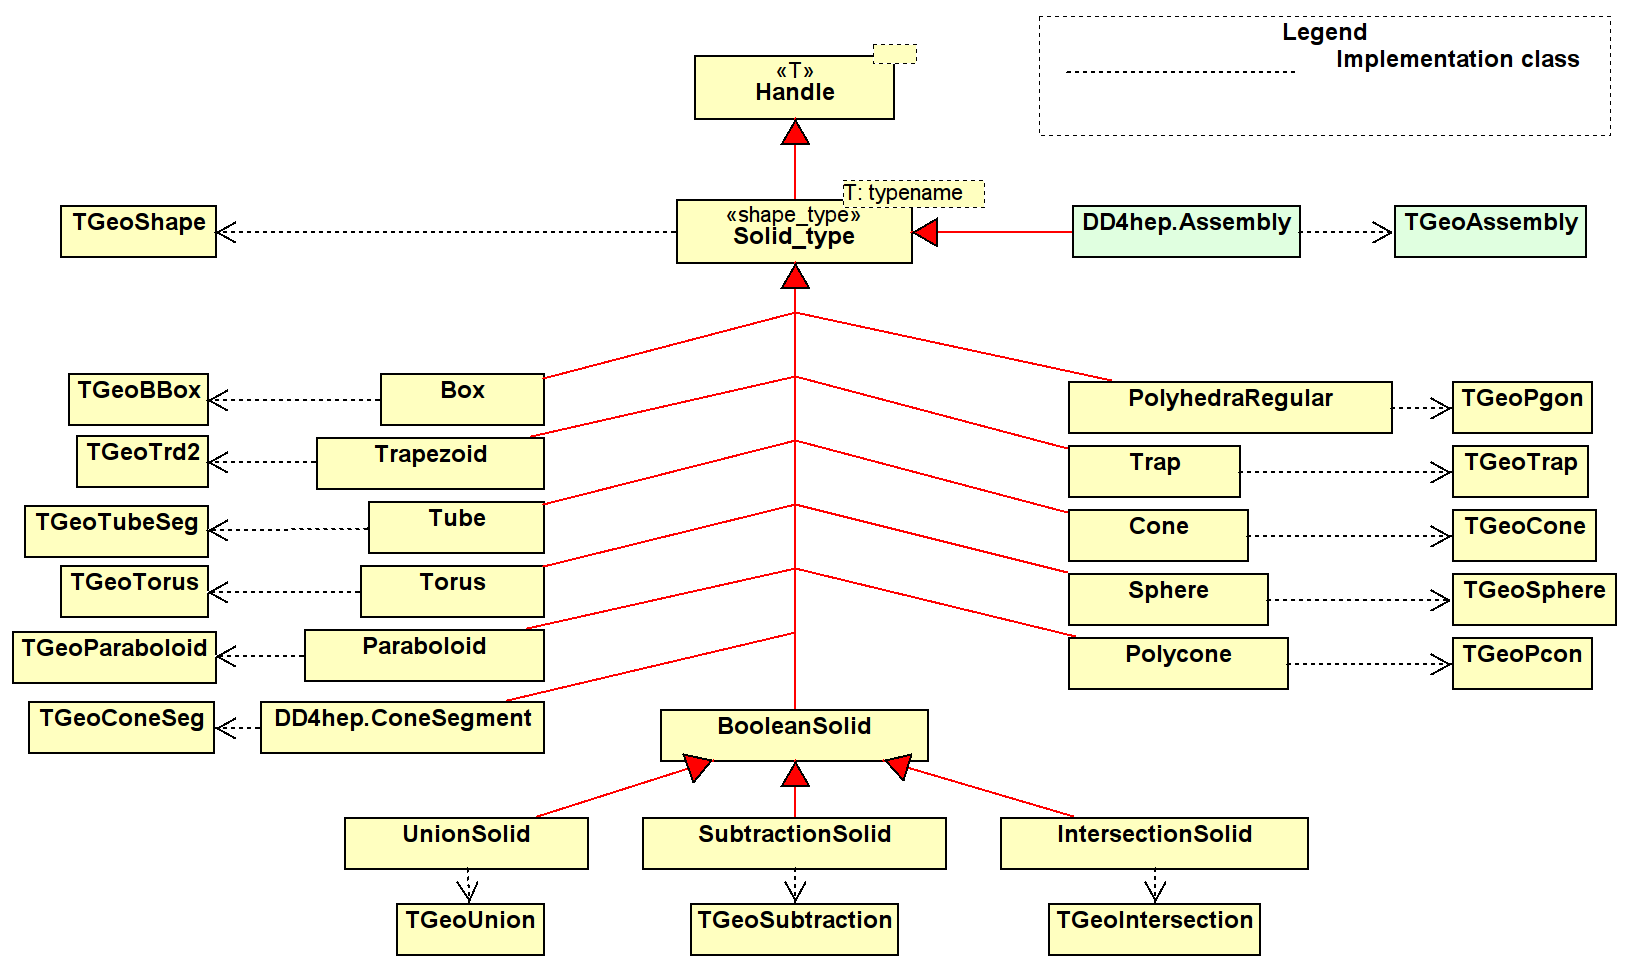
\includegraphics[width=160mm] {DD4hep-solids.png}
    \caption{Extensions may be attached to common Detector Elements which 
             extend the functionality of the common DetElement 
             class and support e.g. caching of precomputed values.}
    \label{fig:dd4hep-solids}
  \end{center}
  \vspace{-0.6cm}
\end{figure}
%=============================================================================
\subsection{Shapes}
\label{dd4hep-basic-shapes}
%=============================================================================
\noindent
Shapes are abstract objects with a bounding surface and fixed dimensions. 
There are primitive, atomic shapes
and complex boolean shapes as shown in Figure~\ref{fig:dd4hep-solids}. 
TGeo and similarly Geant4 offer a whole palette of
primitive shapes, which can be used to construct more complex shapes:
\begin{itemize}\itemcompact
\item \detdesc{html/struct_d_d4hep_1_1_geometry_1_1_box.html}{Box} shape
    represented by the \tgeo{TGeoBBox}{\tt TGeoBBox} class. To create a new box
    object call one of the following constructors:
\begin{code}
/// Constructor to be used when creating an anonymous new box object
Box(double x, double y, double z);
/// Constructor to be used when creating an anonymous new box object
template<typename X, typename Y, typename Z> Box(const X& x, const Y& y, const Z& z);
\end{code}
\item \detdesc{html/struct_d_d4hep_1_1_geometry_1_1_sphere.html}{Sphere} shape
    represented by the \tgeo{TGeoSphere}{\tt TGeoSphere} class. To create a new sphere
    object call one of the following constructors:
\begin{code}
\end{code}
\item \detdesc{html/struct_d_d4hep_1_1_geometry_1_1_cone.html}{Cone}  shape
    represented by the \tgeo{TGeoCone}{\tt TGeoCone} class. To create a new cone
    object call one of the following constructors:
\begin{code}
/// Constructor to create a new anonymous object with attribute initialization
Cone(double z,double rmin1,double rmax1,double rmin2,double rmax2);
template<typename Z, typename RMIN1, typename RMAX1, typename RMIN2, typename RMAX2>
Cone(const Z& z, const RMIN1& rmin1, const RMAX1& rmax1, const RMIN2& rmin2, const RMAX2& rmax2);
\end{code}
\item \detdesc{html/struct_d_d4hep_1_1_geometry_1_1_cone_segment.html}{Cone segment} shape
    represented by the \tgeo{TGeoConeSeg}{\tt TGeoConeSeg} class. To create a new cone segment
    object call one of the following constructors:
\begin{code}
/// Constructor to create a new ConeSegment
ConeSegment(double dz, double rmin1, double rmax1, double rmin2, double rmax2, 
            double phi1=0.0, double phi2=2.0*M_PI);
\end{code}
\item \detdesc{html/struct_d_d4hep_1_1_geometry_1_1_polycone.html}{Polycone}  shape
    represented by the \tgeo{TGeoPcon}{\tt TGeoPcon} class. To create a new polycone
    object call one of the following constructors:
\begin{code}
/// Constructor to create a new polycone object
Polycone(double start, double delta);
followed by a call to:
void addZPlanes(const std::vector<double>& rmin, 
                const std::vector<double>& rmax,
                const std::vector<double>& z);
/// Constructor to create a new polycone object. Add at the same time all Z planes
Polycone(double start, double delta, 
         const std::vector<double>& rmin, 
         const std::vector<double>& rmax, 
         const std::vector<double>& z);
\end{code}
\item \detdesc{html/struct_d_d4hep_1_1_geometry_1_1_tube.html}{Tube segment} shape
    represented by the \tgeo{TGeoTubeSeg}{\tt TGeoTubeSeg} class. To create a new tube segment
    object call one of the following constructors:
\begin{code}
Tube(double rmin, double rmax, double z, double deltaPhi=2*M_PI)
Tube(double rmin, double rmax, double z, double startPhi, double deltaPhi)

template<typename RMIN, typename RMAX, typename Z, typename DELTAPHI>
Tube(const RMIN& rmin, const RMAX& rmax, const Z& z, const DELTAPHI& deltaPhi)  

template<typename RMIN, typename RMAX, typename Z, typename STARTPHI, typename DELTAPHI>
Tube(const std::string& name, const RMIN& rmin, const RMAX& rmax, const Z& z, 
     const STARTPHI& startPhi, const DELTAPHI& deltaPhi)  
\end{code}
\item \detdesc{html/struct_d_d4hep_1_1_geometry_1_1_trapezoid.html}{Trapezoid} shape
    represented by the \tgeo{TGeoTrd2}{\tt TGeoTrd} class. To create a new trapezoid
    object call one of the following constructors:
\begin{code} 
/// Constructor to create a new anonymous object with attribute initialization
Trapezoid(double x1, double x2, double y1, double y2, double z);
\end{code}
\item \detdesc{html/struct_d_d4hep_1_1_geometry_1_1_trap.html}{Trap} shape
    represented by the \tgeo{TGeoTrap}{\tt TGeoTrap} class. To create a new trap
    object call one of the following constructors:
\begin{code} 
/// Constructor to create a new anonymous object with attribute initialization
Trap(double z,double theta,double phi,
     double y1,double x1,double x2,double alpha1,
     double y2,double x3,double x4,double alpha2);
/// Constructor to create a new anonymous object for right angular wedge from STEP (Se G4 manual for details)
Trap( double pz, double py, double px, double pLTX);
\end{code}
\item \detdesc{html/struct_d_d4hep_1_1_geometry_1_1_torus.html}{Torus}  shape
    represented by the \tgeo{TGeoTorus}{\tt TGeoTorus} class. To create a new torus
    object call one of the following constructors:
\begin{code}
/// Constructor to create a new anonymous object with attribute initialization
Torus(double r, double rmin, double rmax, double phi=M_PI, double delta_phi=2.*M_PI);
\end{code}
\item \detdesc{html/struct_d_d4hep_1_1_geometry_1_1_paraboloid.html}{Paraboloid}  shape
    represented by the \tgeo{TGeoParaboloid}{\tt TGeoParaboloid} class. To create a new paraboloid
    object call one of the following constructors:
\begin{code}
/// Constructor to create a new anonymous object with attribute initialization
Paraboloid(double r_low, double r_high, double delta_z);
\end{code}
\item \detdesc{html/struct_d_d4hep_1_1_geometry_1_1_polyhedra_regular.html}{Regular Polyhedron} shape
    represented by the \tgeo{TGeoPgon}{\tt TGeoPgon} class. To create a new polyhedron
    object call one of the following constructors:
\begin{code}
/// Constructor to create a new object. Phi(start)=0, deltaPhi=2PI, Z-planes at +-zlen/2
PolyhedraRegular(int nsides, double rmin, double rmax, double zlen);
/// Constructor to create a new object. Phi(start)=0, deltaPhi=2PI, Z-planes at zplanes[0],[1]
PolyhedraRegular(int nsides, double rmin, double rmax, double zplanes[2]);
/// Constructor to create a new object with phi_start, deltaPhi=2PI, Z-planes at +-zlen/2
PolyhedraRegular(int nsides, double phi_start, double rmin, double rmax, double zlen);
\end{code}
\end{itemize}

\noindent
Besides the primitive shapes three types of boolean shapes (described in TGeo by the
\tgeo{TGeoCompositeShape}{{\tt{TGeoCompositeShape}}} class)
are supported:

\begin{itemize}\itemcompact
\item \detdesc{html/struct_d_d4hep_1_1_geometry_1_1_union_solid.html}{\tt UnionSolid} objects representing the union,
\item \detdesc{html/struct_d_d4hep_1_1_geometry_1_1_intersection_solid.html}{\tt IntersectionSolid} objects representing the intersection,
\item \detdesc{html/struct_d_d4hep_1_1_geometry_1_1_subtraction_solid.html}{\tt SubtractionSolid} objects representing the subtraction,
\end{itemize}

\noindent
of two other primitive or complex shapes. To build a boolean shape, the 
second shape is transformed in 3-dimensional space before the boolean 
operation is applied. The 3D transformations are described by objects from the 
ROOT::Math library and are supplied at construction time. 
Such a transformation as shown in the code snippet below may be 

\begin{itemize}\itemcompact
\item The identity transformation. Then no transformation object needs to be provided (see line 2).

\item A translation only described by a \tw{Position} object (see line 4)

\item A 3-fold rotation first around the Z-axis, then around the Y-axis and finally around the X-axis.
       For transformation operations of this kind a \tw{RotationZYX} object must be supplied (see line 6).

\item A generic 3D rotation matrix should be applied to the second shape. Then a \tw{Rotation3D}
       object must be supplied (see line 8).

\item Finally a generic 3D transformation (translation+rotation) may be applied using a 
       \tw{Transform3D} object (see line 10).
\end{itemize}

\noindent
All three boolean shapes
have constructors as shown here for the UnionSolid:
\begin{code}
  /// Constructor to create a new object. Position is identity, Rotation is identity-rotation!
  UnionSolid(const Solid& shape1, const Solid& shape2);
  /// Constructor to create a new object. Placement by position, Rotation is identity-rotation!
  UnionSolid(const Solid& shape1, const Solid& shape2, const Position& pos);
  /// Constructor to create a new object. Placement by a RotationZYX within the mother
  UnionSolid(const Solid& shape1, const Solid& shape2, const RotationZYX& rot);
  /// Constructor to create a new object. Placement by a generic rotoation within the mother
  UnionSolid(const Solid& shape1, const Solid& shape2, const Rotation3D& rot);
  /// Constructor to create a new object. Placement by a generic transformation within the mother
  UnionSolid(const Solid& shape1, const Solid& shape2, const Transform3D& pos);
\end{code}

\paragraph{Shape factories} Sometimes it is useful to create shapes in an "abstract" way
e.g. to define areas in the detector. To create such shapes a factory method was implemented,
which allows to create a valid shape handle given a valid XML element providing the 
required attributes. The factory methods are invoked using from XML elements of the following form:
\begin{unnumberedcode}
  <some_element type="shape-type" .... args ....>
\end{unnumberedcode}
The shape is then constructed using the XML component object:
\begin{unnumberedcode}
#include "DD4hep/DetFactoryHelper.h"

  xml_h e = <shape-element>;
  Box box = xml_comp_t(e).createShape();
  if ( !box.isValid() ) { ...handle error ... }
\end{unnumberedcode}
The required arguments for the various shapes are then:
\begin{itemize}
\item For a Box:
\vspace{-0.2cm}
\begin{unnumberedcode}
  <some_element type="Box" x="x-value" y="y-value" z="z-value"/>
\end{unnumberedcode}
fulfiling a constructor of the type: $Box(dim.dx(),~dim.dy(),~dim.dz())$.

\item For a Polycone:
\vspace{-0.2cm}
\begin{unnumberedcode}
  <some_element type="Polycone" start="start-phi-value" deltaphi="delta-phi-value">
    <zplane z="z-value" rmin="rmin-value" rmax="rmax-value"/>
    <zplane z="z-value" rmin="rmin-value" rmax="rmax-value"/>
    .... any number of Z-planes ....
    <zplane z="z-value" rmin="rmin-value" rmax="rmax-value"/>
  </some_element>
\end{unnumberedcode}

\item For a ConeSegment the following constructor must be fulfilled:\\
  $ ConeSegment(e.rmin(0.0),~e.rmax(),~e.z(0.0),~e.startphi(0.0),~e.deltaphi(2*M\_PI))$,\\
where the above default values for the XML attributes $rmin, z, startphi$ and 
$deltaphi$ are used if not explicitly stated in the XML element $e$.

\item For a Tube the constructor is:\\
  $ Tube(e.rmin(0.0),~e.rmax(),~e.z(0.0),~e.startphi(0.0),~e.deltaphi(2*M\_PI))$.

\item For a Cone the constructor is:\\
  $double rmi1 = e.rmin1(0.0), rma1 = e.rmax1();$\\
  $ Cone(e.z(0.0),~rmi1,rma1,~e.rmin2(rmi1),~e.rmax2(rma1))$.

\item For a Trap the constructor is:\\
  if $dz$ is specified: $ Trap(e.dz(),~e.dy(),~e.dx(),_toDouble(_Unicode(pLTX)))$
  Otherwise: \\
  $ Trap(e.z(0.0),~e.theta(),~e.phi(0),~e.y1(),~e.x1(),~e.x2(),~e.alpha(),
                    e.y2(),~e.x3(),~e.x4(),~e.alpha2())$.

\item For a Trapezoid the constructor is:\\
  $ Trapezoid(e.x1(),~e.x2(),~e.y1(),~e.y2(),~e.z(0.0))$.

\item For a Torus the constructor is:\\
  $ Torus(e.r(),~e.rmin(),~e.rmax(),~e.phi(M\_PI),~e.deltaphi(2.*M\_PI))$.

\item For a Sphere the constructor is:\\
  $ Sphere(e.rmin(),~e.rmax(),~e.deltatheta(M\_PI),~e.phi(0e0),e.deltaphi(2.*M\_PI))$.

\item For a Paraboloid the constructor is:\\
  $ Paraboloid(e.rmin(0.0),~e.rmax(),~e.dz())$.

\item For a PolyhedraRegular the constructor is:\\
  $ PolyhedraRegular(e.numsides(),~e.rmin(),~e.rmax(),~e.dz())$.

\end{itemize}

\newpage
%=============================================================================
\subsection{Volumes and Placements}
%=============================================================================
\noindent
The detector geometry is described by a hierarchy of volumes and their 
corresponding placements. Both, the TGeo package and Geant4~\cite{bib:geant4} 
are following effectively the same ideas ensuring an easy conversion from 
TGeo to Geant4 objects for the simulation application.
\noindent
A volume is an unplaced solid de\-scribed in terms of a primitive 
shape or a boolean operation of solids, a material and a number of
placed sub-volumes (placed volumes) inside. The class diagram showing the 
relationships between volumes and placements, solids and materials is shown 
in Figure~\ref{fig:dd4hep-detector-model}.
\noindent
It is worth noting, that any volume has children, but no parent or "mother"
volume. This is a direct consequence of the requirement to re-use volumes
and place the same volume arbitrarily often. Only the act of placing a volume
defines the relationship to the next level parent volume.
The resulting geometry tree is very effective, simple and convenient to 
describe the detector geometry hierarchy starting from the top level volume
representing e.g. the experiment cavern down to the very detail of the detector
e.g. the small screw in the calorimeter. The top level volume is the very only
volume without a placement. All geometry calculations, computations are always 
performed within the local coordinate system of the volume.
The following example code shows how to create
a volume which consists of a given material and with a shape. The created volume 
is then placed inside the mother-volume using the local coordinate system of the
mother volume:

\begin{code}
  Volume       mother = ....ampercent

  Material     mat    (lcdd.material("Iron"));
  Tube         tub    (rmin, rmax, zhalf);
  Volume       vol    (name, tub, mat);
  Transform3D  tr     (RotationZYX(rotz,roty,rotx),Position(x,y,z));
  PlacedVolume phv = mother.placeVolume(vol,tr);
\end{code}

\noindent
The volume has the shape of a tube and consists of iron.
Before being placed, the daughter volume is transformed within
the mother coordinate system according to the requested transformation.
The example also illustrates how to access $Material$ objects from the
$LCDD$ interface.

\noindent
The {\tt{Volume}} class provides several possibilities to declare
the required space transformation necessary to place a daughter volume 
within the mother:
\begin{itemize}\itemcompact
\item to place a daughter volume unrotated at the origin of the mother, the 
transformation is the identity. Use the following call to place the daughter:
\begin{unnumberedcode}
PlacedVolume placeVolume(const Volume& vol)  const;
\end{unnumberedcode}
\item If the positioning is described by a simple translation, use:
\begin{unnumberedcode}
PlacedVolume placeVolume(const Volume& vol, const Position& pos)  coampercentnst;
\end{unnumberedcode}
\item In case the daughter should be rotated first around the Z-axis, 
       then around the Y-axis and finally around the X-axis place the daughter 
       using this call:
\begin{unnumberedcode}
PlacedVolume placeVolume(const Volume& vol, const RotationZYX& rot)  const;
\end{unnumberedcode}
\item If the full 3-dimensional rotation matrix is known use:
\begin{unnumberedcode}
PlacedVolume placeVolume(const Volume& vol, const Rotation3D& rot)  const;
\end{unnumberedcode}
\item for an entirely unconstrained placement place the daughter providing
      a Transform3D object:
\begin{unnumberedcode}
PlacedVolume placeVolume(const Volume& volume, const Transform3D& tr)  const;
\end{unnumberedcode}
\end{itemize}

\noindent
For more details of the \tw{Volume} and the \tw{PlacedVolume} classes please see the 
\detdesc{html/_volumes_8h.html}{header file}.

\noindent
One volume like construct is special: the assembly constructs.
Assemblies are volumes without shapes. The "assembly" shape does not
own a own surface by itself, but rather defines it's surface and 
bounding box from the contained children.
In this corner also the implementation concepts between TGeo and Geant4 diverge.
Whereas TGeo handles assemblies very similar to real volumes, in Geant4 
assemblies are purely artificial and disappear at the very moment volumes 
are placed.

\newpage
%=============================================================================
\subsection{Detector Elements}
\label{sec:dd4hep-user-manual-detector-elements}
%=============================================================================
\begin{figure}[b]
  \begin{center}
    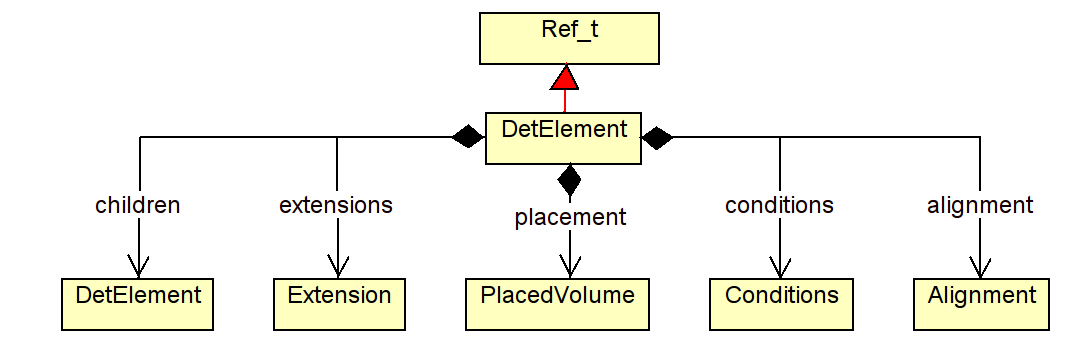
\includegraphics[width=160mm] {DD4hep-detelement-drawing.png}
    \caption{The basic layout of the \tw{DetElement} class aggregating
        all data entities necessary to process data.}
    \label{fig:dd4hep-user-manual-detelement-drawing}
  \end{center}
  \vspace{-0.6cm}
\end{figure}

\noindent
Detector elements (class \tw{DetElement}) are entities which represent 
subdetectors or sizable parts of a subdetector.
As shown in Figure~\ref{fig:dd4hep-user-manual-detelement-drawing},
a \tw{DetElement} instance has the means to provide to clients information about

\begin{itemize}\itemcompact
\item generic properties like the detector type or the path within the \tw{DetElement}s
    hierarchy:
\begin{code}
  /// Access detector type (structure, tracker, calorimeter, etc.).
  std::string type() const;
  /// Path of the detector element (not necessarily identical to placement path!)
  std::string path() const;
\end{code}

\item the detector hierarchy by exposing its children. The hierarchy may be 
    accessed with the following API:
\begin{code}
  /// Add new child to the detector structure
  DetElement& add(DetElement sub_element);
  /// Access to the list of children
  const Children& children() const;
  /// Access to individual children by name
  DetElement child(const std::string& name) const;
  /// Access to the detector elements's parent
  DetElement parent() const;
\end{code}

\item its placement within the overall experiment if it represents an 
    entire subdetector or its placement with respect to its parent
    if the \tw{DetElement} represents a part of a subdetector.
    The placement path is the fully qualified path of placed volumes 
    from the top level volume to the placed detector element and may
    serve as a shortcut for the alignment implementation:
\begin{code}
  /// Access to the full path to the placed object
  std::string placementPath() const;
  /// Access to the physical volume of this detector element
  PlacedVolume placement() const;
  /// Access to the logical volume of the daughter placement
  Volume volume() const;
\end{code}

\item information about the environmental conditions etc. (\tw{conditons}):
\begin{code}
  /// Access to the conditions information 
  Conditions conditions() const;
\end{code}

\item alignment information:
\begin{code}
  /// Access to the alignment information
  Alignment alignment() const;
\end{code}

\item convenience information such as cached transformations
    to/from the top level volume, to/from the parent \tw{DetElement}
    and to/from another \tw{DetElement} in the hierarchy above:
\begin{code}
  /// Transformation from local coordinates of the placed volume to the world system
  bool localToWorld(const Position& local, Position& global) const;
  /// Transformation from world coordinates of the local placed volume coordinates
  bool worldToLocal(const Position& global, Position& local) const;

  /// Transformation from local coordinates of the placed volume to the parent system
  bool localToParent(const Position& local, Position& parent) const;
  /// Transformation from world coordinates of the local placed volume coordinates
  bool parentToLocal(const Position& parent, Position& local) const;

  /// Transformation from local coordinates of the placed volume to arbitrary parent system set as reference
  bool localToReference(const Position& local, Position& reference) const;
  /// Transformation from world coordinates of the local placed volume coordinates
  bool referenceToLocal(const Position& reference, Position& local) const;

  /// Set detector element for reference transformations. 
  /// Will delete existing reference transformation.
  DetElement& setReference(DetElement reference);
\end{code}

\item User extension information as described in section~\ref{sec:dd4hep-user-manual-data-extensions}:
\begin{code}
  /// Extend the detector element with an arbitrary structure accessible by the type
  template <typename IFACE, typename CONCRETE> IFACE* addExtension(CONCRETE* c);
  /// Access extension element by the type
  template <class T> T* extension() const;
\end{code}

\end{itemize}


\newpage
%=============================================================================
\subsection{Sensitive Detectors}
\label{sec:dd4hep-user-manual-sensitive-detectors}
%=============================================================================

\noindent
Though the concept of sensitive detectors comes from Geant4 and simulation 
activities, in DD4hep the sensitive detectors are the client interface to 
access the readout description (class \tw{Readout}) with its 
segmentation of sensitive elements (class \tw{Segmentation}) and
the description of hit decoders (class \tw{IDDescriptors}).
As shown in Figure~\ref{fig:dd4hep-sensitive-detectors}, these object 
instances are required when reconstructing data from particle collisions.

\noindent
Besides the access to data necessary for reconstruction the sensitive detector
also hosts Region setting (class \tw{Region} and sets of cut limits
(class \tw{LimitSets}) used to configure the Geant4 simulation toolkit.
The following code snippet shows the accessors of the 
\tw{SensitiveDetector} class to obtain the corresponding 
information~\footnote{The methods to set the data are not shown here.}:


\vspace{0.3cm}
\begin{code}
    struct SensitiveDetector: public Ref_t {
      /// Access the hits collection name
      const std::string& hitsCollection() const;
      /// Access readout structure of the sensitive detector
      Readout readout() const;
      /// Access to the region setting of the sensitive detector (not mandatory)
      Region region() const;
      /// Access to the limit set of the sensitive detector (not mandatory).
      LimitSet limits() const;

      /// Extend the sensitive detector element with an arbitrary structure accessible by the type
      template <typename IFACE, typename CONCRETE> IFACE* addExtension(CONCRETE* c);
      /// Access extension element by the type
      template <class T> T* extension() const;
   };
\end{code}

\begin{figure}[h]
  \begin{center}
    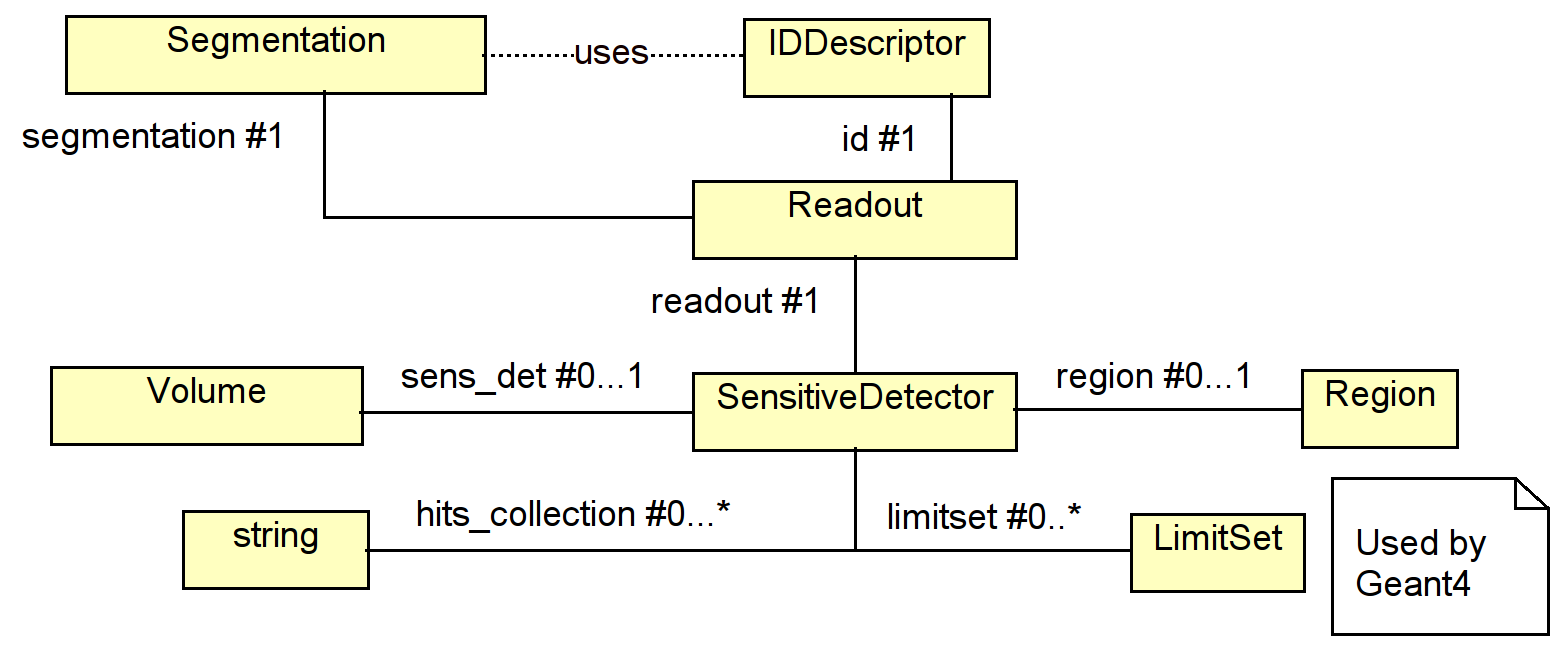
\includegraphics[width=140mm] {DD4hep-sensitive-detectors.png}
    \caption{The structure of DD4hep sensitive detectors.}
    \label{fig:dd4hep-sensitive-detectors}
  \end{center}
  \vspace{-0.6cm}
\end{figure}


\noindent
Sensitive detector objects are automatically creating using the information
of the \tw{<readout>} section of the XML file if a subdetector is sensitive
and references a valid readout entry.
In the detector constructor (or any time later) clients 
may add additional information to a sensitive detector object using 
an extension mechanism similar to the extension mechanism for 
detector elements mentioned earlier.


\noindent
Volumes may be shared and reused in several placements. In the parallel
hierarchy of detector elements as shown in Figure~\ref{fig:dd4hep-hierarchies},
the detector elements may reference unambiguously the volumes of their 
respective placements, but not the reverse.
However, the sensitive detector setup is a single instance per subdetector.
Hence it may be referenced by all sensitive Volumes of one subdetector.
In the following chapters the access to the readout structure is described.

%=============================================================================
\subsection{Description of the Readout Structure}
\label{sec:dd4hep-manual-readout-description}
%=============================================================================
\noindent
The \tw{Readout} class describes the detailed structure of a sensitve volume.
The for example may be the layout of strips or pixels in a silicon detector
i.e. the description of entities which would not be modeled using individual
volumes and placements though this would theoretically  feasible.
Each sensitive element is segmented according to the \tw{Segmentation} object 
and hits resulting from energy depositions in the sensitive volume are 
encoded using the \tw{IDDescriptor} object.

\begin{figure}[h]
  \begin{center}
    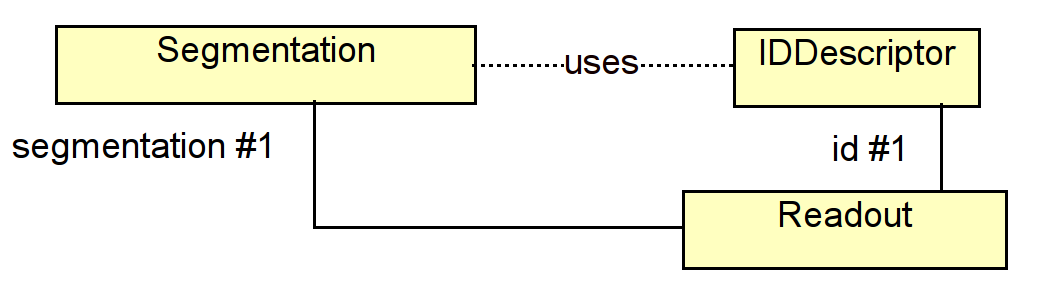
\includegraphics[width=100mm] {DD4hep-readout.png}
    \caption{The basic components to describe the \tw{Readout} structure
    of a subdetector. }
    \label{fig:dd4hep-sensitive-detectors}
  \end{center}
  \vspace{-0.6cm}
\end{figure}

%=============================================================================
\subsubsection{CellID Descriptors}
\label{sec:dd4hep-manual-readout-iddescriptors}
%=============================================================================
\noindent
\tw{IDDescriptor}s define the encoding of sensitive volumes to uniquely identify
the location of the detector response. The encoding defines a bit-field with
the length of 64 bits. The first field is mandatory called \tw{system} and 
identifies the subdetector. All other fields define the other volumes in the 
hierarchy. The high bits are not necessarily mapped to small daughter volumes,
but may simply identify a logical segmentation such as the \tw{strip} \tw{number}
within a wafer of a vertex detector as shown in the following XML snippet:
\begin{code}
<readouts>
  <readout name="SiVertexEndcapHits">
    <id>system:8,barrel:3,layer:4,module:14,sensor:2,side:32:-2,strip:24</id>
  </readout>
<readouts>
\end{code}
These identifiers are the data input to 
\tw{segmentation classes}~\ref{sec:dd4hep-manual-readout-segmentations},
which define a user friendly API to en/decode the detector response.

%=============================================================================
\subsubsection{Segmentations}
\label{sec:dd4hep-manual-readout-segmentations}
%=============================================================================
\noindent
Segementations define the user API to the low level interpretation of
the energy deposits in a subdetector. For technical reasons and partial
religious reasons are the segmentation implementation not part of the \DDhep 
toolkit, but an independent package call 
\tw{DDSegmentation}~\cite{bib:DDSegmentations}. Though the usage is an 
integral part of DD4hep.

\subsubsection{Volume Manager}
%=============================================================================
\noindent
The \tw{VolumeManager} is a tool to seek a lookup table of placements of 
sensitive volumes and their corresponding unique volume identifier, the 
\tw{cellID}. The volume manager analyzes - once the geometry is closed -
the hierarchical tree and stores the various placements in the hierarchy 
with respect to their identifiers. In other words the the tree is 
reused volumes shown e.g. in Figure~\ref{fig:dd4hep-hierarchies} is 
degenerated  according to the full pathes of the various volumes. This 
use case is very common to reconstruction and analysis applications
whenever a given raw-data (aka "hit") element must be related to its
geometrical location.

\noindent
Figure~\ref{fig:dd4hep-user-manual-volmgr} shows the design diagram of this component:
\begin{figure}[h]
  \begin{center}
    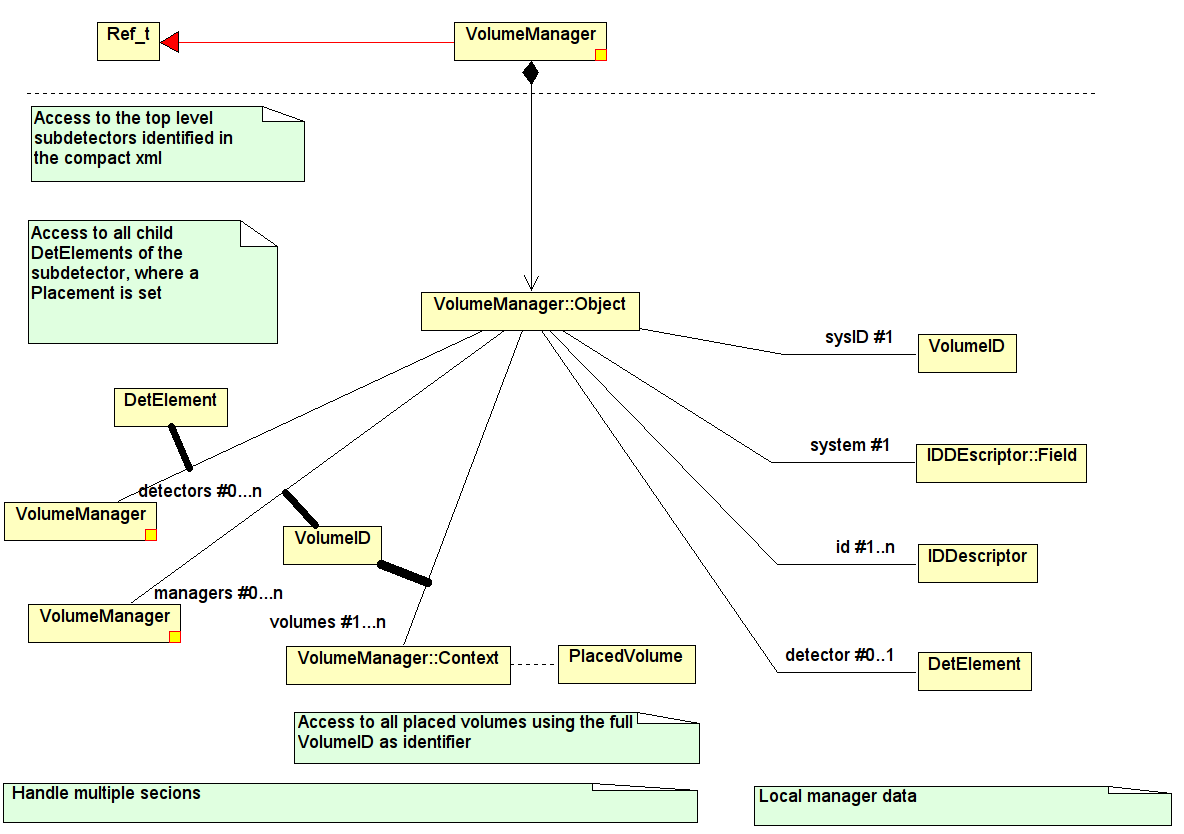
\includegraphics[width=170mm] {DD4hep-volmgr.png}
    \caption{Extensions may be attached to common Detector Elements which 
             extend the functionality of the common DetElement 
             class and support e.g. caching of precomputed values.}
    \label{fig:dd4hep-user-manual-volmgr}
  \end{center}
\end{figure}

\noindent
To optimize the access of complex subdetector structures, is the volume-identifier
map split and the volumes of each each subdetector is stored in a separate map.
This optimization however is transparent to clients. The following code extract
from the header files lists the main client routines to extract volume information
given a known cellID:
\begin{code}
  /// Lookup the context, which belongs to a registered physical volume.
  Context* lookupContext(VolumeID volume_id) const;
  /// Lookup a physical (placed) volume identified by its 64 bit hit ID
  PlacedVolume lookupPlacement(VolumeID volume_id) const;
  /// Lookup a top level subdetector detector element 
  /// according to a contained 64 bit hit ID
  DetElement lookupDetector(VolumeID volume_id) const;
  /// Lookup the closest subdetector detector element in the hierarchy 
  /// according to a contained 64 bit hit ID
  DetElement lookupDetElement(VolumeID volume_id) const;
  /// Access the transformation of a physical volume to the world coordinate system
  const TGeoMatrix& worldTransformation(VolumeID volume_id) const;
\end{code}

%=============================================================================
\subsubsection{Static Electric and Magnetic Fields}
\label{sec:dd4hep-manual-static-fields}

\noindent
The generic field is described by a structure of any field type (electric or magnetic)
with field components in Cartesian coordinates.
The overlay field is the sum of several magnetic of electric field components
and the resulting field vectors are computed by the vector addition 
of the individual components. The available components are described in the following.
If necessary new field implementations may be added at any time: they are 
instantiated when necessary by the factory mechanism.
Fields are described in the compact model within the {\tt{<fields>}} tags the 
following examople shows:
\begin{code}
  <fields>
    <field name="MyMagnet" type="solenoid"  .... />
  </fields>
\end{code}
The actual components are defined one by one within the {\tt{<field>}} tags.

\paragraph{Constant Electric or Magnetic Fields} are defined as follows:
\begin{code}
  <field  name="MyMagnet" type="ConstantField" field="electric">
    <strength x="x-val" y="y-val" z="z-val"/>
  </field>
\end{code}
The {\tw{field}} attribute accepts take the values {\tw{[electric,magnetic]}}
depending on it's nature.

\paragraph{Magnetic Dipoles} are defined as follows:
\begin{code}
  <field name="MyMagnet" type="DipoleMagnet"
         rmax="50*cm"
         zmin="0*cm"
         zmax="50*cm">
         <dipole_coeff>1.0*tesla</dipole_coeff>
         <dipole_coeff>0.1*tesla/pow(cm,1)</dipole_coeff>
         <dipole_coeff>0.01*tesla/pow(cm,2)</dipole_coeff>
  </field>
\end{code}

\paragraph{Magnetic Multipole Fields} are developed according to their 
approximation using the multipole coefficients.
The dipole is assumed to be horizontal as it is used for bending beams in large colliders
ie. the dipole field lines are vertical.

The different momenta are given by:  $ B_y + i  B_x $\footnote{
See for detailed documentation about multipoles:\\
http://cas.web.cern.ch/cas/Belgium-2009/Lectures/PDFs/Wolski-1.pdf \\
http://cas.web.cern.ch/cas/Bulgaria-2010/Talks-web/Brandt-1-web.pdf \\
https://en.wikipedia.org/wiki/Multipole\_magnet
}, where:
\begin{align*}
        & & B_y + i B_x &=& C_n (x + iy)^{n-1}                         \\
B_{sum} &=& B_y + i B_x &=& \Sigma_{n=1..m} (b_n + ia_n) (x + iy)^{n-1}\\
\end{align*}
With $C_n$ being the complex multipole coefficients,
$b_n$ the "normal multipole coefficients" and $a_n$ the "skew multipole coefficients".
The maximal momentum used is the octopole momentum. The lower four momenta are used
to describe the magnetic field:
\begin{itemize}\itemcompact
\item Dipole (n=1):
    \begin{align*}
        B_y &=& b_1                                       \\
        B_x &=& a_1                                       \\
        B_z &=& constant                                  \\
    \end{align*}
\item Quadrupole (n=2):
    \begin{align*}
        B_y &=& b_2 x - a_2 y                             \\
        B_x &=& b_2 y + a_2 x                             \\
    \end{align*}
\item Sextupole (n=3):
    \begin{align*}
        B_y + i B_x &=& (b_3 +ia_3) (x^2 + 2ixy - y^2)    \\
        B_y         &=& b_3 x^2 - b_3 y^2 - 2 a_3 xy      \\
        B_x         &=& a_3 x^2 - a_3 y^2 + 2 b_3 xy      \\
    \end{align*}

\item Octopole (n=4):
    \begin{align*}
        B_y + i B_x &=& (b_4 +ia_4) (x^3 + 3ix^2y - 3xy^2 -iy^3)  \\
        B_y &=& b_4 x^3 - 3 b_4 x y^2 - 3 a_4 x^2 y + a_4 y^3     \\
        B_x &=& 3 b_4 x^2 y + b_4 y^3 + a_4 x^3 - 3 a_4 x y^2     \\
    \end{align*}
\end{itemize}
The defined field components only apply within the shape 'volume'.
If 'volume' is an invalid shape (ie. not defined), then the field
components are valied throughout the 'universe'.

\noindent
The magnetic multipoles are defined as follows:
\begin{code}
  <field name="MyMagnet" type="MultipoleMagnet">
         <position x="0" y="0" z="0"/>
         <rotation x="pi" y="0" z="0"/>
         <shape type="shape-constructor-type" .... args .... >
         <coeffizient coefficient="coeff(n=1)" skew="skew(n=1)"/>
           .... maximum of 4 coefficients ....
         <coeffizient coefficient="coeff(n=4)" skew="skew(n=4)"/>
  </field>
\end{code}
The shape defines the geometrical coverage of the multipole 
field in the origin (See section~\ref{dd4hep-basic-shapes} for details). 
This shape may then be transformed to
the required location in the detector area using the position 
and the rotation elements, which define this transformation.

\newpage
%=============================================================================
\subsection{Detector Constructors}
\label{sec:dd4hep-manual-detector-constructors}
%=============================================================================
\noindent
The creation of appropriate detector constructors is the main work of a client
defining his own detector. The detector constructor is a fragment of code in the 
form of a routine, which return a handle to the created subdetector 
\tw{DetElement} object.

\noindent
Knowing that detector constructors are the main work items of clients significant 
effort was put in place to ease and simplify this procedure as much as possible
in order to obtain readable, still compact code hopefully easy to maintain.
The interfaces to all objects, XML accessors, shapes, volumes etc. which were 
discussed above were optimized to support this intention.

\noindent
To illustrate the anatomy of such a constructor the following code originating
from an existing SiD detector concept will be analyzed. The example starts
with the XML input data. Further down this section the code is shown 
with a detailed description of every relevant line. The object to be build is 
a subdetector representing a layered calorimeter, 
where each layer consists of a number of slices as shown in the XML snippet. 
These layers are then repeated a number of times.

\vspace{0.1cm}
\noindent
The XML snippet describing the subdetector properties:
\begin{code}
  <detector id="13" name="LumiCal" reflect="true" type="CylindricalEndcapCalorimeter" 
            readout="LumiCalHits" vis="LumiCalVis" calorimeterType="LUMI">
    <comment>Luminosity Calorimeter</comment>
    <dimensions inner_r = "LumiCal_rmin" inner_z = "LumiCal_zmin" outer_r = "LumiCal_rmax" />
    <layer repeat="20" >
      <slice material = "TungstenDens24" thickness = "0.271*cm" />
      <slice material = "Silicon" thickness = "0.032*cm" sensitive = "yes" />
      <slice material = "Copper"  thickness = "0.005*cm" />
      <slice material = "Kapton"  thickness = "0.030*cm" />
      <slice material = "Air"     thickness = "0.033*cm" />
    </layer>
    <layer repeat="15" >
      <slice material = "TungstenDens24" thickness = "0.543*cm" />
      <slice material = "Silicon" thickness = "0.032*cm" sensitive = "yes" />
      <slice material = "Copper"  thickness = "0.005*cm" />
      <slice material = "Kapton"  thickness = "0.030*cm" />
      <slice material = "Air"     thickness = "0.033*cm" />
    </layer>
  </detector>
\end{code}

\vspace{0.1cm}
\noindent
The C++ code snippet interpreting the XML data and expanding the geometry:
\vspace{0.1cm}
\begin{code}
#include "DD4hep/DetFactoryHelper.h"
#include "XML/Layering.h"

using namespace std;
using namespace DD4hep;
using namespace DD4hep::Geometry;

static Ref_t create_detector(LCDD& lcdd, xml_h e, SensitiveDetector sens)  {
  xml_det_t  x_det     = e;
  string     det_name  = x_det.nameStr();
  bool       reflect   = x_det.reflect();
  xml_dim_t  dim       = x_det.dimensions();
  double     zmin      = dim.inner_z();
  double     rmin      = dim.inner_r();
  double     rmax      = dim.outer_r();
  double     totWidth  = Layering(x_det).totalThickness();
  double     z         = zmin;
  Material   air       = lcdd.air();
  Tube       envelope   (rmin,rmax,totWidth,0,2*M_PI);
  Volume     envelopeVol(det_name+"_envelope",envelope,air);
  int        layer_num = 1;
  PlacedVolume pv;

  // Set attributes of slice
  for(xml_coll_t c(x_det,_U(layer)); c; ++c)  {
    xml_comp_t x_layer = c;
    double layerWidth = 0;
    for(xml_coll_t l(x_layer,_U(slice)); l; ++l)
      layerWidth += xml_comp_t(l).thickness();

    for(int i=0, m=0, repeat=x_layer.repeat(); i<repeat; ++i, m=0)  {
      double     zlayer = z;
      string     layer_name = det_name + _toString(layer_num,"_layer%d");
      Volume     layer_vol(layer_name,Tube(rmin,rmax,layerWidth),air);
        
      for(xml_coll_t l(x_layer,_U(slice)); l; ++l, ++m)  {
        xml_comp_t x_slice = l;
        double     w = x_slice.thickness();
        string     slice_name = layer_name + _toString(m+1,"slice%d");
        Material   slice_mat  = lcdd.material(x_slice.materialStr());
        Volume     slice_vol (slice_name,Tube(rmin,rmax,w),slice_mat);
          
        if ( x_slice.isSensitive() )  {
          sens.setType("calorimeter");
          slice_vol.setSensitiveDetector(sens);
        }
        slice_vol.setAttributes(lcdd,x_slice.regionStr(),x_slice.limitsStr(),x_slice.visStr());
        pv = layer_vol.placeVolume(slice_vol,Position(0,0,z-zlayer-layerWidth/2+w/2));
        pv.addPhysVolID("slice",m+1);
        z += w;
      }
      layer_vol.setVisAttributes(lcdd,x_layer.visStr());
      Position layer_pos(0,0,zlayer-zmin-totWidth/2+layerWidth/2);
      pv = envelopeVol.placeVolume(layer_vol,layer_pos);
      pv.addPhysVolID("layer",layer_num);
      ++layer_num;
    }
  }
  // Set attributes of slice
  envelopeVol.setAttributes(lcdd,x_det.regionStr(),x_det.limitsStr(),x_det.visStr());

  DetElement   sdet(det_name,x_det.id());
  Volume       motherVol = lcdd.pickMotherVolume(sdet);
  PlacedVolume phv = motherVol.placeVolume(envelopeVol,Position(0,0,zmin+totWidth/2));
  phv.addPhysVolID("system",sdet.id())
     .addPhysVolID("barrel",1);
  sdet.setPlacement(phv);
  if ( reflect )   {
    phv=motherVol.placeVolume(envelopeVol,Transform3D(RotationZ(M_PI),Position(0,0,-zmin-totWidth/2)));
    phv.addPhysVolID("system",sdet.id())
      .addPhysVolID("barrel",2);
  }
  return sdet;
}

DECLARE_DETELEMENT(CylindricalEndcapCalorimeter,create_detector);
\end{code}

\newpage
\noindent
\begin{tabular} {l||p{0cm}}
\docline{Line}{}
\docline{1}{The include file DetFactoryHelper.h includes all
    utilities to extract XML information together with the appropriate type 
    definition.}
\docline{4-6}{Convenience shortcut to save ourself a lot of typing.}
\docline{8}{The entry point to the detector constructor. This routine shall 
    be called by the plugin mechanism.}
\docline{9}{The functionality of the raw XML handle \tw{xml\_h} is rather 
    limited. A simple assignment to a XML detector object gives us all the 
    functionality we need.}
\docline{10,11}{Extracting the sub-detector name and properties from the xml handle.}
\docline{12-17}{Access the $dimension$ child-element from the XML subtree, access the element's 
    attributes and precompute values used later.}
\docline{18}{Retrieve a reference to the "air" material from LCDD.}
\docline{19-20}{Construct the envelope volume shaped as a tube made out of air.}
\docline{25}{Now the detector can be built: We loop over all layers types and over
              each layer type as often as necessary (attribute: repeat).
              The XML collection object will return all child elements of \tw{x\_det}
              with a tag-name "layer".             }
\docline{25}{Note the macro $\tt{\_U(layer)}$: When using Xerces-C as an XML parser, 
    it will expand to the reference to an object containing the unicode value 
    of the string "layer". The full list of predefined tag names can be found in the
    include file \detdesc{html/_unicode_values_8h.html}{DD4hep/UnicodeValues.h}.
    If a user tag is not part in the precompiled tag list, the corresponding Unicode
    string may be created with the macro \tw{\_Unicode(layer)} or \tw{Unicode("layer")}.
    }
\docline{26}{Convenience assignment to extract attributes of the layer element.}
\docline{27-29}{Compute total layer width.}
\docline{31}{Create \tw{repeat} number of layers of the same type.}
\docline{32-34}{Create the named envelope volume with a tube shape 
    containing all slices of this layer.}
\docline{36-51}{Create the different layer-slices with a tube shape and the 
    corresponding material as indicated in the XML data.}
\docline{43-46}{If the slice is sensitive i.e. is instrumented and supposed to 
    deliver signals from particle passing, the sensitive detector component of this
    detector needs to be attached to the slice.}
\docline{47}{Set visualization and geant4 attributes to the slice volume. 
    If the attributes are not present, they will be ignored.}
\docline{48}{Now the created slice volume will be placed inside the mother, 
    the layer envelope at the correct position. This operation results 
    in the creation of a \tw{PlacedVolume}.}
\docline{49}{It identify uniquely every slice within the layer an identifier 
    (here the number of the created slice) is attached. This identifier 
    must be present in the
    bitmap defined by the \tw{IDDescriptor} of this subdetector.}
\docline{52-55}{Same as 47-49, but now the created layer volume is placed 
    in the envelope of the entire subdetector.}
\docline{60}{Set envelope attributes.}
\docline{62}{Construct the main detector element of this subdetector.
    This will be the unique entry point to access any information of the subdetector.\\
    {\bf{Note:}} the subdetector my consist of a hierarchy of detector elements.
    For example each layer could be described by it's own \tw{DetElement} and all
    layer-\tw{DetElement} instances being children of the subdetector instance.
    }
\docline{63-64}{Place the subdetector envelope into its mother 
    (typically the top level (world) volume).}
\docline{65-66}{Add the missing \tw{IDDescriptor} identifiers to complete the bitmap.}
\docline{67}{Store the placement in the subdetector detector 
    element in order to make it availible to later clients of this \tw{DetElement}.}
\end{tabular}
\newpage
\begin{tabular} {l||p{0cm}}
\docline{Line}{}
\docline{68-72}{Endcap calorimeters typically are symmetric i.e. an 
    endcap is located on each side of the barrel. To easy such 
    reflections the entire endcap structure 
    can be copied and placed again. }
\docline{73}{All done. Return the created subdetector element to the caller for registration.}
\docline{76}{{\bf Very important:}Without the registration of the construction 
    function to the framework, the corresponding plugin will not be found.
    The macro has two arguments: firstly the plugin name which is identical to the
    detector type in the XML snippet and secondly the function to be called
    at construction time.}
\end{tabular}

\newpage
%=============================================================================
\subsection{Tools and Utilities}

%=============================================================================
\subsubsection{Geometry Visualization}
\label{sec:dd4hep-manual-geometry-visualization}
%=============================================================================
\noindent
Visualizing the geometry is an important tool to debug and validate
the constructed detector.
Since \DDhep uses the \tw{ROOT} geometry package, all visualization tools
from ROOT are automatically supported. This is in the first place the 
OpenGL canvas of \tw{ROOT} and all elaborated derivatives thereof such as 
event displays etc. Figure~\ref{fig:dd4hep-user-manual-visualization-subdetector}
shows as an example the subdetector example from the \tw{SiD} detector design
discussed in section~\ref{sec:dd4hep-manual-detector-constructors}.
\begin{figure}[h]
  \begin{center}
    \begin{tabular}{l r}
      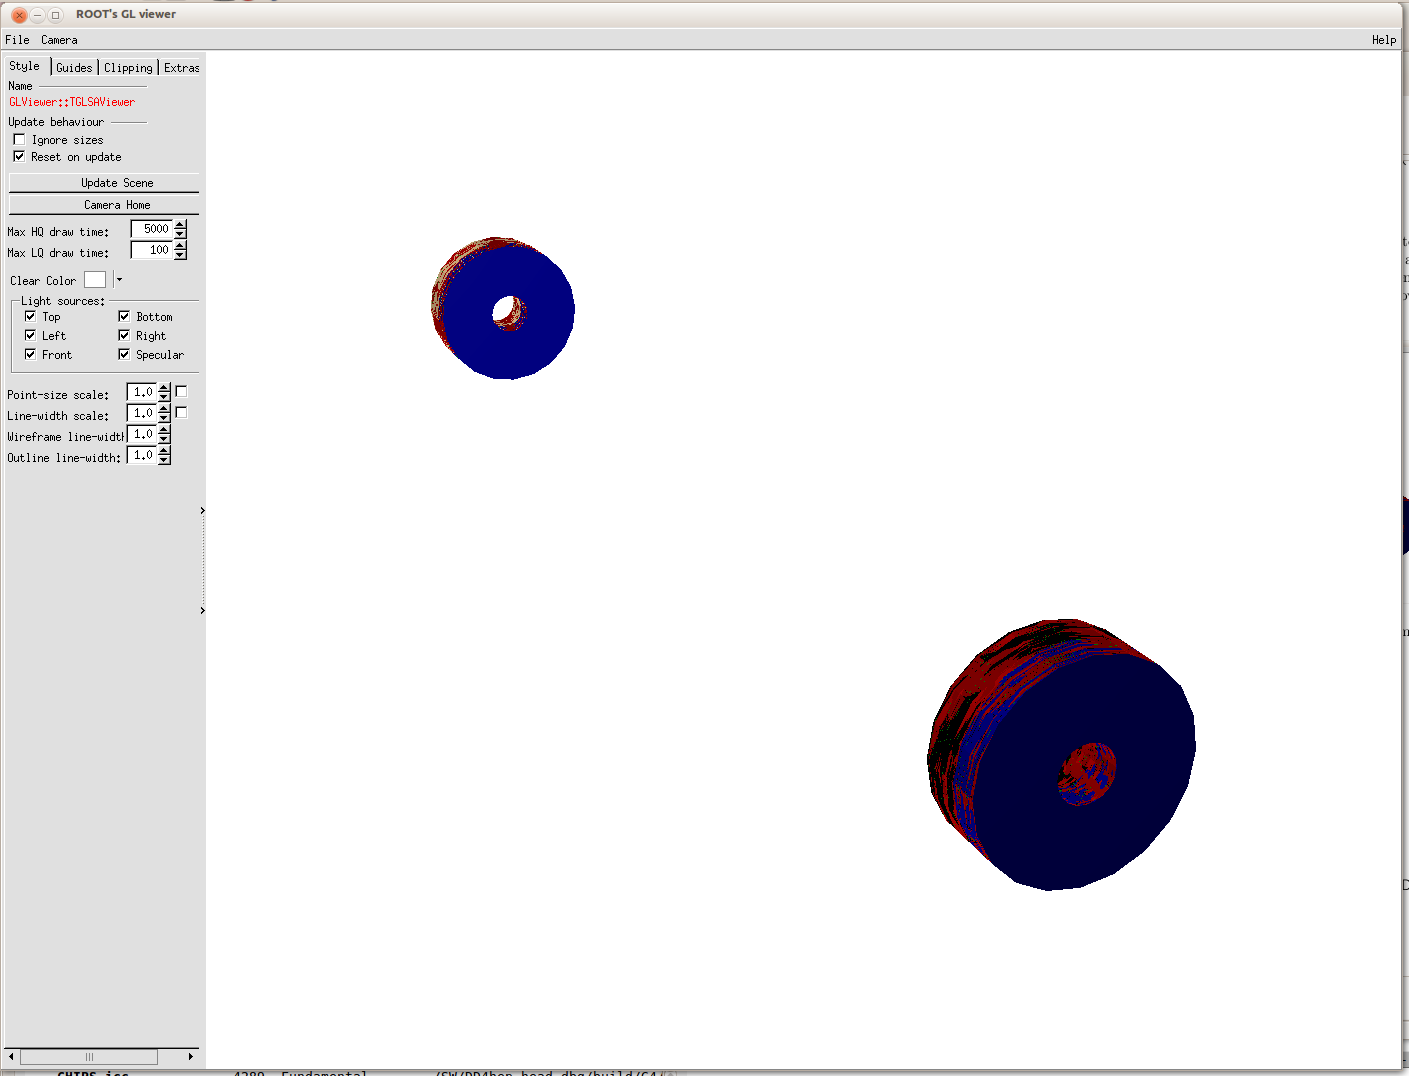
\includegraphics[width=80mm] {DD4hep-Lumical.png} &
      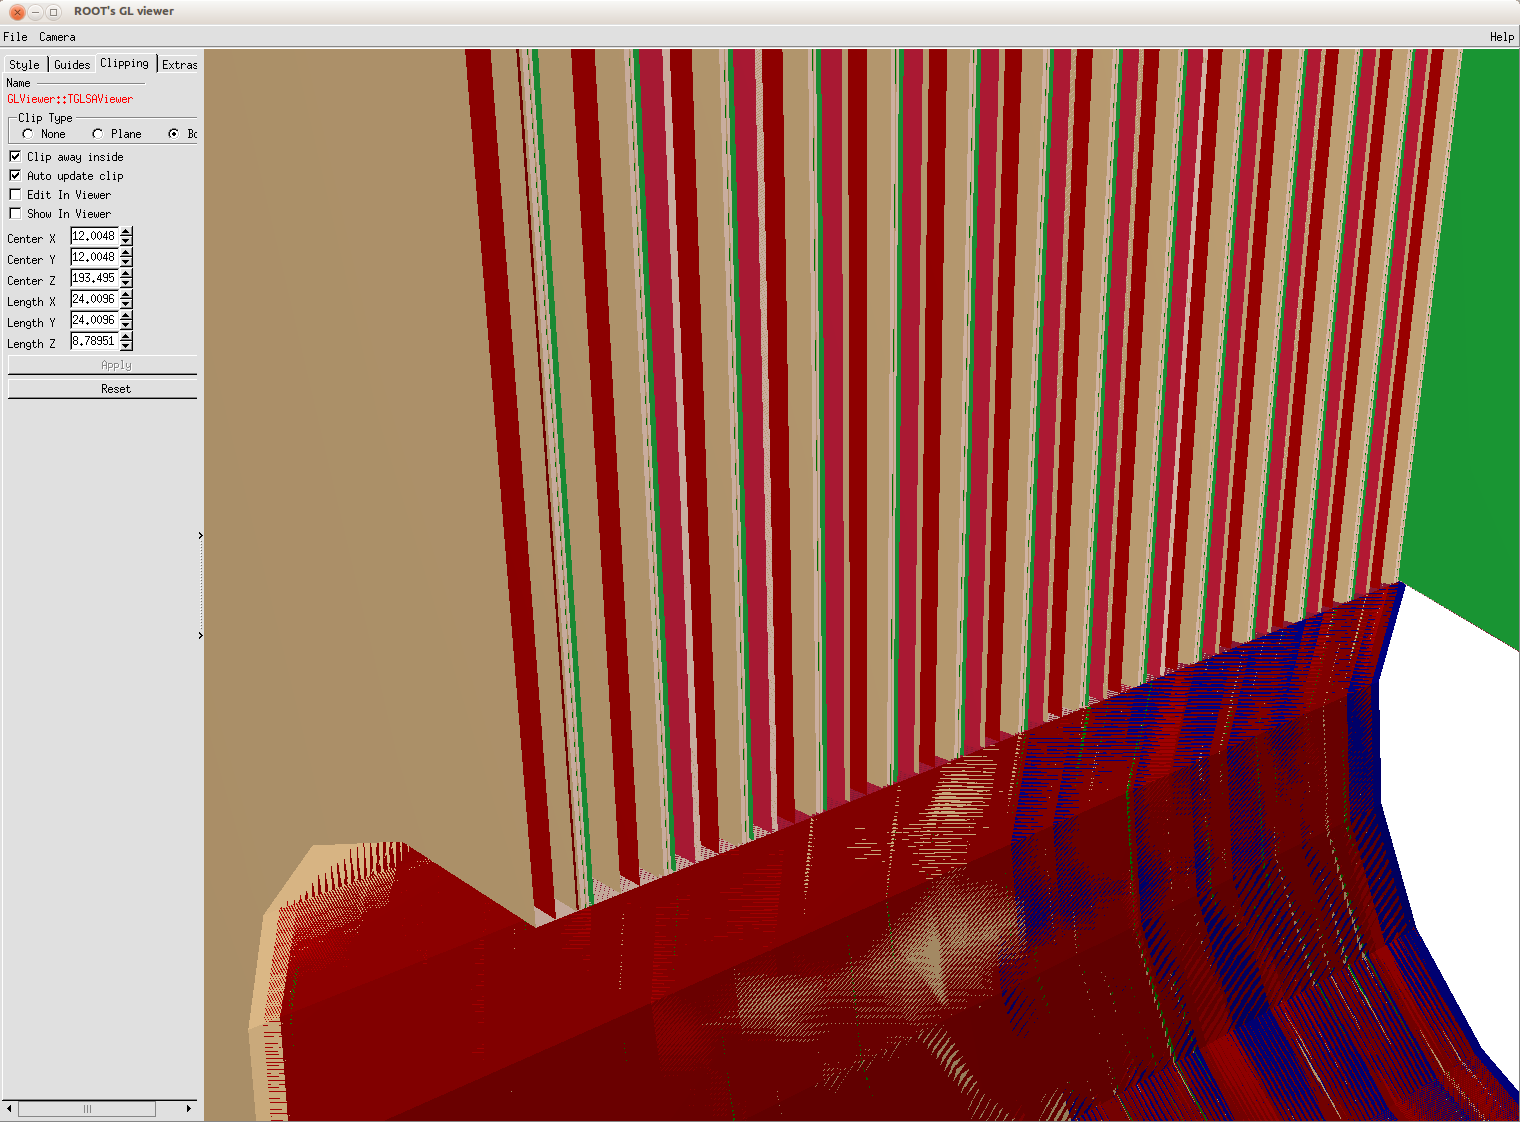
\includegraphics[width=80mm] {DD4hep-Lumical-detailed.png} \\
    \end{tabular}
    \caption{Geometry visualization using the ROOT OpenGL plugin.
        To the left the entire luminosity calorimeter is shown,
        at the right the detailed zoomed view with clipping to 
        access the internal layer and slice structure.}
    \label{fig:dd4hep-user-manual-visualization-subdetector}
  \end{center}
\end{figure}

\noindent
The command to create the display is part of the DD4hep release:
\begin{code}
$> geoDisplay -compact <path to the XML file containing the detector description>

 DD4hepGeometryDisplay -opt [-opt]                                                  
        -compact       <file>       Specify the compact geometry file              
                     [REQUIRED]     At least one compact geo file is required!     
        -build_type <number/string> Specify the build type                         
                     [OPTIONAL]     MUST come immediately after the -compact input.
                                    Default for each file is: BUILD_DEFAULT [=1]   
                                    Allowed values: BUILD_SIMU [=1], BUILD_RECO [=2] or BUILD_DISPLAY [=3]
        -destroy     [OPTIONAL]     Force destruction of the LCDD instance         
                                    before exiting the application                 
        -volmgr      [OPTIONAL]     Load and populate phys.volume manager to       
                                    check the volume ids for duplicates etc.       
        -print      <number/string> Specify output level. Default: INFO(=3)        
                     [OPTIONAL]     Allowed values: VERBOSE(=1), DEBUG(=2),        
                                    INFO(=3), WARNING(=4), ERROR(=5), FATAL(=6)    
                                    The lower the level, the more printout...      
        -load_only   [OPTIONAL]     Dry-run to only load geometry without     
                                    starting the dispay.                      
\end{code}

%=============================================================================
\subsubsection{Geometry Conversion}
\label{sec:dd4hep-manual-geometry-conversion}
%=============================================================================
\noindent
\tw{ROOT} \tw{TGeo} is only one representation of a detector geometry.
Other applications may require other representation. In particular two other
are worth mentioning:
\begin{itemize}\itemcompact
\item \tw{LCDD}~\cite{bib:LCDD} the geometry representation used to 
    simulate the ILC detector design with the \tw{slic} application.
\item \tw{GDML}~\cite{bib:GDML} a geometry markup language understood
    by Geant4 and \tw{ROOT}.
\end{itemize}
Both conversions are supported in \DDhep with the geoConverter application:
\begin{code}
  geoConverter -opt [-opt]                                                
        Action flags:               Usage is exclusive, 1 required!           
        -compact2lcdd               Convert compact xml geometry to lcdd.     
        -compact2gdml               Convert compact xml geometry to gdml.     
        -compact2vis                Convert compact xml to visualisation attrs

        -input  <file>  [REQUIRED]  Specify input file.                       
        -output <file>  [OPTIONAL]  Specify output file.                      
                                    if no output file is specified, the output
                                    device is stdout.                         
        -ascii          [OPTIONAL]  Dump visualisation attrs in csv format.   
                                    [Only valid for -compact2vis]             
\end{code}

%=============================================================================
\subsubsection{Overlap checking}
\label{sec:dd4hep-manual-overlap-checking}
%=============================================================================
\noindent
Overlap checks are an important tool to verify the consistency of the 
implemented geometrical design. As in the real world, where overlaps are 
impossible, also simulated geometries may not have overlaps. In simulation
overlaps tend to create particle reflections possibly leading to infinite
loops.
\begin{code}
    python <install>/DD4hep/bin/checkOverlaps.py --help
    Usage: checkOverlaps.py [options]

    Check TGeo geometries for overlaps.

    Options:
      -h, --help                        show this help message and exit
      -c <FILE>, --compact=<FILE>       Define LCCDD style compact xml input
      -p <boolean>, --print=<boolean>   Print overlap information to standard output
                                        (default:True)
      -q, --quiet                       Do not print (disable --print)
      -t <double number>, --tolerance=<double number>
                                        Overlap checking tolerance. Unit is in [mm].
                                        (default:0.1 mm)
      -o <string>, --option=<string>    Overlap checking option ('' or 's')
\end{code}

%=============================================================================
\subsubsection{Geometry checking}
\label{sec:dd4hep-manual-geometry-checking}
%=============================================================================
\noindent
Perform extensive geometry checks. For details and up to date information 
please refer to the ROOT documentation of the class {\tt{TGeoManager}}:
\begin{itemize}\itemcompact
\item Member function {\tgeoO{TGeoManager.html}{TGeoManager:CheckGeometry}{TGeoManager::CheckGeometry}} and 
\item Member function {\tgeoO{TGeoManager.html}{TGeoManager:CheckGeometryFull}{TGeoManager::CheckGeometryFull}}
\end{itemize}

\begin{code}
    python <install>DD4hep/bin/checkGeometry.py --help
    Usage: checkGeometry.py [options]

    TGeo Geometry checking.

    Options:
      -h, --help                            show this help message and exit
      -c <FILE>, --compact=<FILE>           Define LCCDD style compact xml input
      -f <boolean>, --full=<boolean>        Full geometry checking
      -n <integer>, --ntracks=<integer>     Number of tracks [requires 'full']
      -x <double>, --vx=<double>            X-position of track origine vertex [requires 'full']
      -y <double>, --vy=<double>            Y-position of track origine vertex [requires 'full']
      -z <double>, --vz=<double>            Z-position of track origine vertex [requires 'full']
      -o <string>, --option=<string>        Geometry checking option default:ob
\end{code}

The full geometry check performs the \tgeoO{TGeoManager.html}{TGeoManager:CheckGeometryFull}
{following actions}:
\begin{itemize}\itemcompact
\item if option contains 'o': Optional overlap checkings (by sampling and by mesh).
\item if option contains 'b': Optional boundary crossing check + timing per volume.

\item{\bf{STAGE 1:}} extensive overlap checking by sampling per volume. Stdout need to be
  checked by user to get report, then TGeoVolume::CheckOverlaps(0.01, "s") can
  be called for the suspicious volumes.
\item{\bf{STAGE 2:}} normal overlap checking using the shapes mesh - fills the list of
  overlaps.
\item{\bf{STAGE 3:}} shooting NTRACKS rays from vertex (vx,vy,vz) 
   and counting the total number of
  crossings per volume (rays propagated from boundary to boundary until
  geometry exit). Timing computed and results stored in a histogram.
\item{\bf{STAGE 4:}} shooting 1 mil. random rays inside EACH volume and calling
  FindNextBoundary() + Safety() for each call. The timing is normalized by the
  number of crossings computed at stage 2 and presented as percentage.
  One can get a picture on which are the most "burned" volumes during
  transportation from geometry point of view. Another plot of the timing per
  volume vs. number of daughters is produced.
\end{itemize}

%=============================================================================
\subsubsection{Directional Material Scans}
\label{sec:dd4hep-manual-directional-material-scans}
%=============================================================================
\noindent
Print the materials on a straight line between the two given points:
\begin{code}
materialScan
 usage: print_materials compact.xml x0 y0 z0 x1 y1 z1 
        -> prints the materials on a straight line between the two given points ( unit is cm) 
\end{code}
$materialScan$ uses the python bindings provided by Geant4 and may be not 
always availible. Alternatively the command $print\_materials$ may be used, 
which does not use the python binding, but produces less pretty output.

%=============================================================================
\subsubsection{Plugin Test Program}
\label{sec:dd4hep-manual-plugin-test}
%=============================================================================
\noindent
The plugin tester loads a given geometry and the executes a plugin
defined at the command line. The main purpose of this program is to quickly 
invoke new detector plugins while developing. The arguments for this 
program are:
\begin{code}
    geoPluginRun -opt [-opt]                                                
    
        -plugin <name>  [REQUIRED]  Plugin to be executed and applied.        
        -input  <file>  [OPTIONAL]  Specify geometry input file.              
        -build_type <number/string> Specify the build type                         
                     [OPTIONAL]     MUST come immediately after the -compact input.
                                    Default for each file is: BUILD_DEFAULT [=1]   
                                    Allowed values: BUILD_SIMU [=1], BUILD_RECO [=2] or BUILD_DISPLAY [=3]
        -destroy     [OPTIONAL]     Force destruction of the LCDD instance         
                                    before exiting the application                 
        -volmgr      [OPTIONAL]     Load and populate phys.volume manager to       
                                    check the volume ids for duplicates etc.       
        -print      <number/string> Specify output level. Default: INFO(=3)        
                     [OPTIONAL]     Allowed values: VERBOSE(=1), DEBUG(=2),        
                                    INFO(=3), WARNING(=4), ERROR(=5), FATAL(=6)    
                                    The lower the level, the more printout...      


\end{code}

%=============================================================================
\newpage
\begin{thebibliography}{9}
\bibitem{bib:DD4hep}  DD4Hep web page, http://aidasoft.web.cern.ch/DD4hep.

\bibitem{bib:LHCb} 		LHCb Collaboration, 
                "LHCb, the Large Hadron Collider beauty experiment, reoptimised detector 
				design and performance", CERN/LHCC 2003-030

\bibitem{bib:LHCb-geometry} S. Ponce et al., 
                "Detector Description Framework in LHCb", 
                International Conference on Computing in High Energy and Nuclear Physics  (CHEP 2003), 
                La Jolla, CA, 2003, proceedings. 

\bibitem{bib:ILD}  The ILD Concept Group, 
                   "The International Large Detector: Letter of Intent",\\
                   ISBN 978-3-935702-42-3, 2009.

\bibitem{bib:SiD}  H. Aihara, P. Burrows, M. Oreglia (Editors),
                   "SiD Letter of Intent",
                   arXiv:0911.0006, 2009.

\bibitem{bib:ROOT-tgeo} R.Brun, A.Gheata, M.Gheata, "The ROOT geometry package",\\
                    Nuclear Instruments and Methods {\bf{A}} 502 (2003) 676-680.

\bibitem{bib:ROOT} R.Brun et al., 
                   "Root - An object oriented data analysis framework",\\
                    Nuclear Instruments and Methods {\bf{A}} 389 (1997) 81-86.

\bibitem{bib:geant4}  S. Agostinelli et al., 
                   "Geant4 - A Simulation Toolkit", \\
                    Nuclear Instruments and Methods {\bf{A}} 506 (2003) 250-303.

\bibitem{bib:LCDD} T.Johnson et al., 
                   "LCGO - geometry description for ILC detectors", 
                   International Conference on Computing in High Energy and Nuclear Physics  (CHEP 2007), 
                   Victoria, BC, Canada, 2012, Proceedings.

\bibitem{bib:lcsim} N.Graf et al., 
                   "lcsim: An integrated detector simulation, 
                   reconstruction and analysis environment", 
                   International Conference on Computing in High Energy and Nuclear Physics (CHEP 2012),
                   New York, 2012, Proceedings.

\bibitem{bib:GDML} R. Chytracek et al.,
                   "Geometry Description Markup Language for Physics Simulation and Analysis
                   Applications",
                   IEEE Trans. Nucl. Sci., Vol. 53, Issue: 5, Part 2, 2892-2896,
                   http://gdml.web.cern.ch.

\bibitem{bib:DDAlign} M.Frank,
                   "DDAlign User Manual: 
                   Alignment Support for the DD4hep Geometry Description Toolkit".
\bibitem{bib:DDSegmentations} C.Grefe et al.,
                   "The DDSegmentation package", 
                   Non existing documentation to be written.
\end{thebibliography}
%=============================================================================
\end{document}
